\documentclass[twoside]{book}
\usepackage[paperwidth=17cm, paperheight=22.5cm, bottom=2.5cm, right=2.5cm]{geometry}
\usepackage{amssymb,amsmath,amsthm} %paquete para símbolo matemáticos
\usepackage[spanish]{babel}
\usepackage[utf8]{inputenc} %Paquete para escribir acentos y otros símbolos directamente
\usepackage{enumerate}
\usepackage{graphicx}
\usepackage{setspace}
\usepackage{float}
\usepackage[nottoc]{tocbibind}
\setcounter{secnumdepth}{3} %para que ponga 1.1.1.1 en subsubsecciones
\setcounter{tocdepth}{3} % para que ponga subsubsecciones en el indice
\usepackage{fancyhdr}
\renewcommand{\baselinestretch}{1.5}
\begin{document}
%\begin{figure}[h] %	
%	%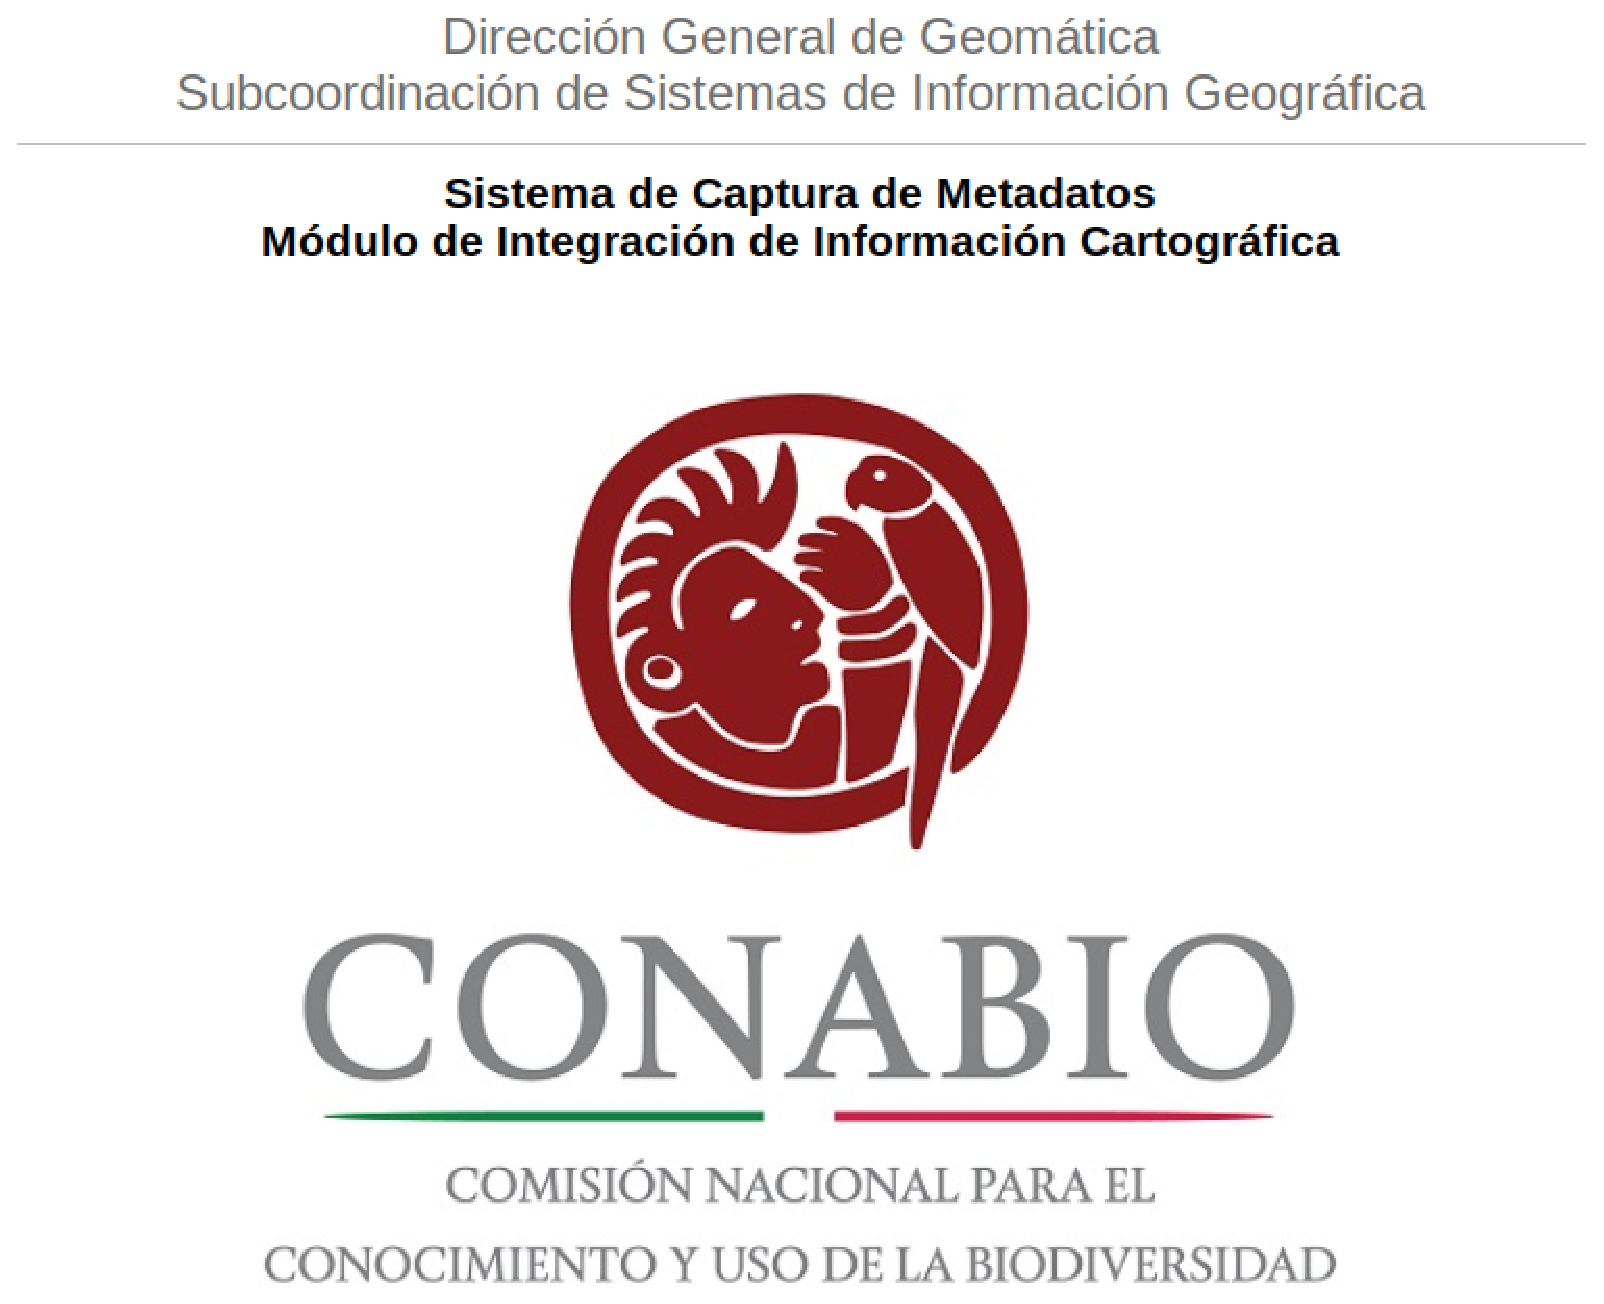
\includegraphics[width=13cm, height=5cm]{img/portada_ssig} %	
%    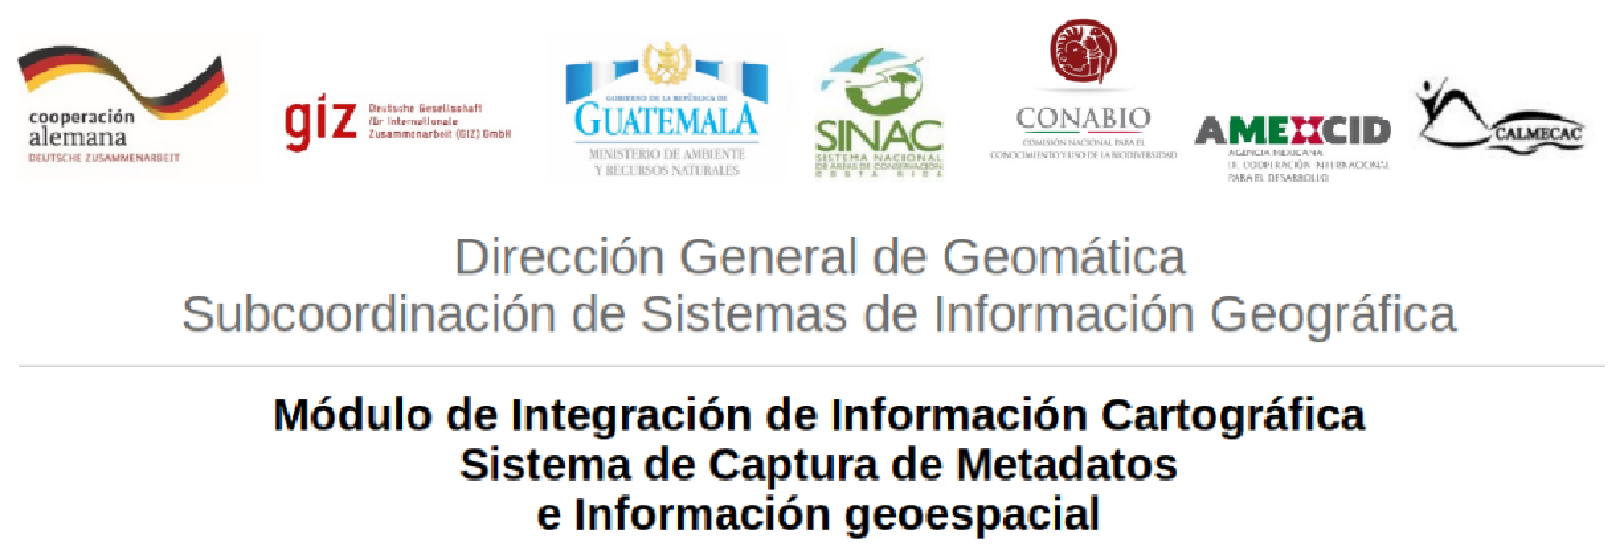
\includegraphics[width=14cm, height=5.5cm]{img/portadaF} %	
%\end{figure}

\title{Manual del\\Sistema de Integración de Información Cartográfica\\e Información Geoespacial\\} %Con este nombre se guardará el proyecto en writeLaTex
%\author{Fís. Gustavo Magallanes Guijón}
\date{}
\thispagestyle{empty}
\maketitle

\thispagestyle{empty}
\setlength{\headheight}{15pt}
\pagestyle{fancy}
\fancyhf{}
\lhead[\thepage]{\textit{\small{\rightmark}}}
\rhead[\textit{\small{\rightmark}}]{\thepage}

\fancyhead[lo]{\slshape\nouppercase{\rightmark}}
\fancyhead[re]{\slshape\nouppercase{\leftmark}}
\frontmatter 

% aqui definimos el pie de pagina de las paginas pares e impares.
\lfoot[\tiny{\textit{Sistema de Integración de Información Cartográfica\\e Información Geoespacial}}]{\tiny{\textit{Comisión Nacional para el Conocimiento y uso de la Biodiversidad\\Corredor Biológico Mesoaméricano}}}
\rfoot[\tiny{\textit{Comisión Nacional para el Conocimiento y uso de la Biodiversidad\\Corredor Biológico Mesoaméricano}}]{\tiny{\textit{Sistema de Integración de Información Cartográfica\\e Información Geoespacial}}}
\renewcommand{\footrulewidth}{0.5pt}

\tableofcontents
\setcounter{tocdepth}{3} % para que ponga subsubsecciones en el indice
\mainmatter %empieza la numeración de las páginas

\chapter*{Introducción}
\addcontentsline{toc}{chapter}{Introducción}
\markboth{Introducción}{Introducción} % encabezado 

\noindent{La Subcoordinación de Sistemas de Información Geográfica (SSIG) de la Comisión Nacional para el Conocimiento y Uso de la Biodiversidad (Conabio), tiene entre sus objetivos: Actualizar y mantener el componente del sistema de información geográfica del Sistema Nacional de Información sobre Biodiversidad (SNIB); así como asegurar la consistencia de la información cartográfica; y compilar, sistematizar y analizar información geográfica, para ayudar en la toma de decisiones derivadas de los resultados de los diferentes proyectos desarrollados en la Comisión. Todo ello con el propósito de proporcionar información geográfica estandarizada y de calidad al personal de la Comisión y público en general. Para cumplir con dichos objetivos y buscando que los datos sean de utilidad al usuario, es necesario documentar la información cartografía a través del manejo de “metadatos geoespaciales”. }

El metadato surge por la necesidad de mejorar la adquisición, distribución, utilización y mapeo de los datos geoespaciales, El metadato se define como la “información acerca de los datos” o “datos de los datos”; que describe el contenido, calidad, condición y referencia espacial de los datos. 

La estructura de los metadatos geoespaciales digitales que maneja la CONABIO sigue el estándar aprobado por el FGDC\footnote{El Comité Federal de Datos Geográficos (FGDC por sus siglas en inglés) se creó en los EEUU para coordinar la Infraestructura Nacional de Datos Espaciales (NSDI, en inglés también).}, que provee un conjunto común de terminologías, definiciones e información acerca de datos geoespaciales. El estándar especifica los elementos necesarios para apoyar el uso de los metadatos en los siguientes puntos: 1) mantener una inversión interna en la organización de los datos geoespaciales; 2) proveer información hacia las agencias distribuidoras de datos y catálogos; y 3) proveer información necesaria para procesar e interpretar la transferencia de datos desde otras organizaciones. Así mismo, proporciona la información requerida por un usuario al determinar (a) la disponibilidad de un dato o conjunto de datos geoespaciales, (b) la propiedad de un dato o conjunto de datos geoespaciales para un uso futuro, (c) la forma de acceso al dato o conjunto de datos geoespaciales y (d) la transferencia exitosa del dato o conjunto de datos geoespaciales.

El estándar se divide en siete secciones:

\begin{enumerate}
\item \textbf{Identificación}: información básica acerca de los datos como título, área incluida, temas, actualidad, restricciones, etcétera.
\item \textbf{Calidad de los datos}: evaluación general de los datos como precisión, metodología, fuentes originales, etcétera.
\item \textbf{Organización de los datos espaciales}: tipo de estructura del dato espacial, vector o raster.
\item \textbf{Referencia espacial}: descripción de la referencia espacial a través de proyección, datum, sistemas de coordenadas, etcétera.
\item \textbf{Entidad y atributos}: descripción del contenido de los datos espaciales como entidades, atributos, dominio de valores de los atributos, etcétera.
\item \textbf{Distribución}: información acerca del distribuidor y las opciones de obtención de los datos geoespaciales como: nombre del distribuidor, formatos, medios, estatus, precio, etcétera.
\item \textbf{Referencia de los metadatos}: nivel de actualización, institución o persona responsable, etcétera.
\end{enumerate}

\chapter{Metadatos Geoespaciales}
%\addcontentsline{toc}{chapter}{Metadatos Geoespaciales}
%\markboth{n}{Introducción} % encabezado 

\noindent{Con base en el estándar de metadatos geoespaciales del FGDC (versión 2.0, 1 mayo 2000), la Subdirección de Sistemas de Información Geográfica (SSIG) elaboró una adecuación adaptando el estándar a las necesidades de la CONABIO, manteniendo el objetivo primordial del estándar que es el de documentar los datos geoespaciales. Para entenderla, a continuación se describen los siguientes puntos:}

\begin{enumerate}
\item Adecuación
\item Secciones
\item Ingreso del dato
\item Descripción de los elementos que componen cada sección
\item Ejemplo de un metadato

\end{enumerate}

Con lo anterior, la Dirección General de Geomática junto con la Subcoordinación de Sistemas de Información Geográfica se han dado la tarea de crear un sistema integral de información cartográfica, el cual consiste en un sistema de captura de metadatos y de un módulo de integración cartográfica. La finalidad es integrar todos los puntos antes dichos de una manera óptima y automatizada, acelerando la generación de metadatos a la vez de poder enfrentar grandes voluménes de informacion.

La dirección electrónica para ingresar sistema es:

http://ssig.conabio.gob.mx:2900/modulo\_cbm


\section{Adecuación}

\noindent{Tomando en cuenta el estándar del FGDC, así como el constante crecimiento de la información cartográfica en la SSIG, como lo es la inclusión de la información cartográfica del Corredor Biológico Mesoamericano en el geoportal de la CONABIO, se decidió usar el gestor de base de datos Postgres, tanto por ser software libre como por su módulo de manejo de información geoespacial Potgis.}

Las secciones que se tomaron para describir los datos geoespaciales, son las que manejan datos obligatorios. Con base en lo anterior, el estándar queda adecuado en tres secciones de la siguiente manera:
\begin{enumerate}
\item Información básica
\item Calidad de los datos
\item Información espacial y atributos
\end{enumerate}
	
La administración de los metadatos se realizará mediante la interfaz web desarrollada para la captura de la información cartográfica.

Dicha interfaz cuenta con un sistema de ventanas que corresponden a: 

\begin{itemize}
	\item Menú inicial.
	\item Ingreso de un nuevo registro.
	\item Selección de  un registro para su edición y las tres secciones enlistadas en el punto anterior (Información básica,  calidad de los datos, e Información espacial y atributos).
\end{itemize}

A continuación se explica el proceso de captura de los datos para la elaboración de los metadatos geoespaciales. Cabe aclarar que el ingreso de un metadato corresponde a la información de un dato geoespacial (archivo vectorial o raster) y dentro de la base de datos a un registro. 

\noindent{\textit{a)} Nuevo Registro}\\
\textit{b)} Duplicar Registro

\section{Nuevo Registro}
\noindent{Esta parte consiste en dar de alta un nuevo registro de metadato.  Para esto se parte de la pestaña de la parte izquierda que dice ``Nuevo registro'' al cual al acceder nos ofrece la opción de ``Crear nuevo Metadato''. Con lo que una vez ingresado el nombre se puede comenzar a agregar la información de los demás campos.}

Es importante decir que una vez generado el metadato no se puede borrar. Se puede editar: cambiar el nombre, atributos, etc. Pero su eliminación corresponde únicamente al Administrador de metadatos.

\section{Duplicar Registro}

\noindent{Como se menciono anteriormente esta herramienta sirve para duplicar una o varias veces un metadato ya terminado, preferentemente, lo cual resulta de mucha ayuda cuando los datos a capturar son muy similares y son pocos los datos que se deben cambiar.}

\textbf{Nota: es importante mencionar que el metadato que se usará para hacer duplicado no contenga información con comillas en alguno de los apartados, ya que si las tiene al momento de hacer el duplicado enviara un mensaje de error.} 

Una vez abierta la sección, dentro del menú inicial ir al botón Duplicar Registro y en la ventana selección del registro de la metabase para editar o revisar, seleccionar el registro que servirá de base para el duplicado.

Aparece una ventana, en el campo geoespacial que se duplicara y en, se anotara el título del dato se anotara el nombre del dato geoespacial (archivo shapefile o raster) (Este nombre no debe tener más de once caracteres y debe ser escrito en mayúsculas), es importante recordar que tanto el título del registro como el nombre del archivo no se pueden repetir.

Una vez capturada la información necesaria presionar el botón Duplicar Metadato.

Si se desea duplicar más de una vez el metadato repetir tantas veces como sean necesarios los pasos anteriores.

\chapter{Información básica}

\noindent{En esta sección se proporcionan los datos mínimos necesarios para que un metadato sea válido y útil al usuario. Se indica el nombre del autor o autores, la escala del mapa, el propósito por el cual se creó, la extensión que abarca, el lugar donde se ubica, etcétera. }
La sección se divide en cinco partes o elementos compuestos que son: Datos Generales, Ubicación Geográfica, Restricciones, Palabras Clave y Ambiente de Trabajo.

A continuación se describen cada uno de los elementos compuestos y sus campos. Es importante que la captura se haga en el orden que se enlistan.
\section{Datos Generales}
\subsection{Título del mapa}
\noindent{Aparece de forma automática al comenzar a editar, y corresponde al nombre del registro que dimos de alta en la ventana Nombrar y salvar un nuevo registro. Esta se realizó desde la selección del registro.}

\subsection{Fecha de Ingreso}
\noindent{Es la fecha de inicio de la captura del metadato. Esta fecha es permanente, por lo que no debe modificarse.}

\subsection{Fecha de actualización}
\noindent{Es la fecha en la que se realiza una actualización o un duplicado del metadato. Ésta, en un principio, será la misma que la fecha de ingreso y será colocada automáticamente por el programa. Solo se modificará si se efectúa una actualización en el dato geoespacial, como la eliminación o adición de elementos geográficos, o eliminación o adición de atributos. Nunca en los casos en los que se reinicie la edición de un registro por no haberse terminado o por correcciones ortográficas o de redacción del metadato.}

\subsection{Nombre del archivo}
\noindent{Es el nombre del archivo que corresponde al dato geoespacial (capa digital). Este nombre no debe tener más de once caracteres y debe ser escrito en mayúsculas.}

\section{Cita de la información}

\subsection{Institución responsable}
\noindent{Es la institución responsable de publicar el dato geoespacial y puede ser la institución donde labora el responsable del proyecto, o bien la CONABIO. Queda a criterio del autor o autores la designación de dicha institución.}

\subsection{Siglas de la institución}
\noindent{Siglas de la institución designada por el autor o autores como la institución responsable de la publicación.}

\subsection{Lugar de publicación}
\noindent{Nombre de la ciudad, estado y país donde se publicará el dato geoespacial. }

\subsection{Versión}
\noindent{Es sinónimo de edición y como sucede con un libro la primera publicación corresponderá a la primera edición, por lo que el valor de este campo dependerá de la edición del dato geoespacial que se está publicando. Si es de primera vez, el valor será 1.}

\subsection{Escala}
\noindent{Corresponde a la escala del dato geoespacial, la cual deberá escribirse como una razón donde el antecedente indica el valor del plano y el consecuente el valor de la realidad: ejemplo, 1:50000, lo que significa que 1 cm en el plano representa 50000 cm o 500 m en la realidad.}

\subsection{Fecha}
\noindent{Es el año de elaboración o modificación del dato geoespacial. }

\subsection{Descripción del metadato}
\noindent{Es un campo donde se aporta información complementaria a la cita del dato geoespacial. Es decir, si fue extraído de algún atlas o proyecto, si fue apoyado por alguna institución como la CONABIO u otros. Y por último, se debe indicar el nombre del proyecto apoyado por la CONABIO a partir del cual se elaboró el dato geoespacial (sólo aplica para los proyectos apoyados por la CONABIO). }

\subsection{Clave}
\noindent{Corresponde a la clave del proyecto asignada por la CONABIO, si aplica.}

\subsection{Autores}
\noindent{Nombre de la o las persona(s) responsables de la elaboración del dato geoespacial. Tomando en cuenta la siguiente estructura; para el primer autor: apellidos seguido de coma, iniciales del o los nombres seguido de un punto; si el autor es una institución sólo se anota la sigla o acrónimo y segundo, tercero o más autores: inicial del o los nombres seguido de un punto; apellidos seguido de una coma.}

\subsection{Resumen}
\noindent{Descripción breve del contenido, área cubierta y tema que representa el dato geoespacial.}

\subsection{Abstract (Resumen en inglés)}
\noindent{Opcional.}

\subsection{Objetivos Generales}
\noindent{Propósito por el cual se creó el dato geoespacial, es decir, el porqué de su creación. No debe confundirse con el o los objetivos de un proyecto en el cual esté inmerso el dato geoespacial.}

\subsection{Datos Complementarios}
\noindent{Información complementaria a cerca del dato geoespacial, que contribuya al entendimiento del porqué de su elaboración, cómo se realizó, etcétera.}

\subsection{Tiempo comprendido}
 \noindent{Información acerca del tiempo que se tomó para elaborar el dato geoespacial.}

 \subsection{Nivel de avance}
\noindent{Grado de avance del dato geoespacial con base en los siguientes vocablos: planeado, en proceso o completo.}

\subsection{Mantenimiento}
\noindent{Frecuencia de actualización del dato geoespacial con base en los siguientes términos: diariamente, semanalmente, mensualmente, anualmente, continuamente, irregularmente, no planeado o desconocido.}

\subsection{Tamaño del Dato Geoespacial en Mb}
\noindent{Tamaño en megabytes del o los archivo(s) que contiene el dato geoespacial.}

\subsection{Formato del Dato Geoespacial}
\noindent{Formato digital del o los archivo(s) que contienen el dato geoespacial. El formato debe corresponder a los estipulados en los lineamientos cartográficos de la CONABIO (documento que describe la forma de cómo entregar Cartografía digital).}

\subsection{Ligas www}
\noindent{En este campo se puede anexar una o varias ligas a páginas Web de interés para los usuarios.}
\begin{figure}[h] %	
    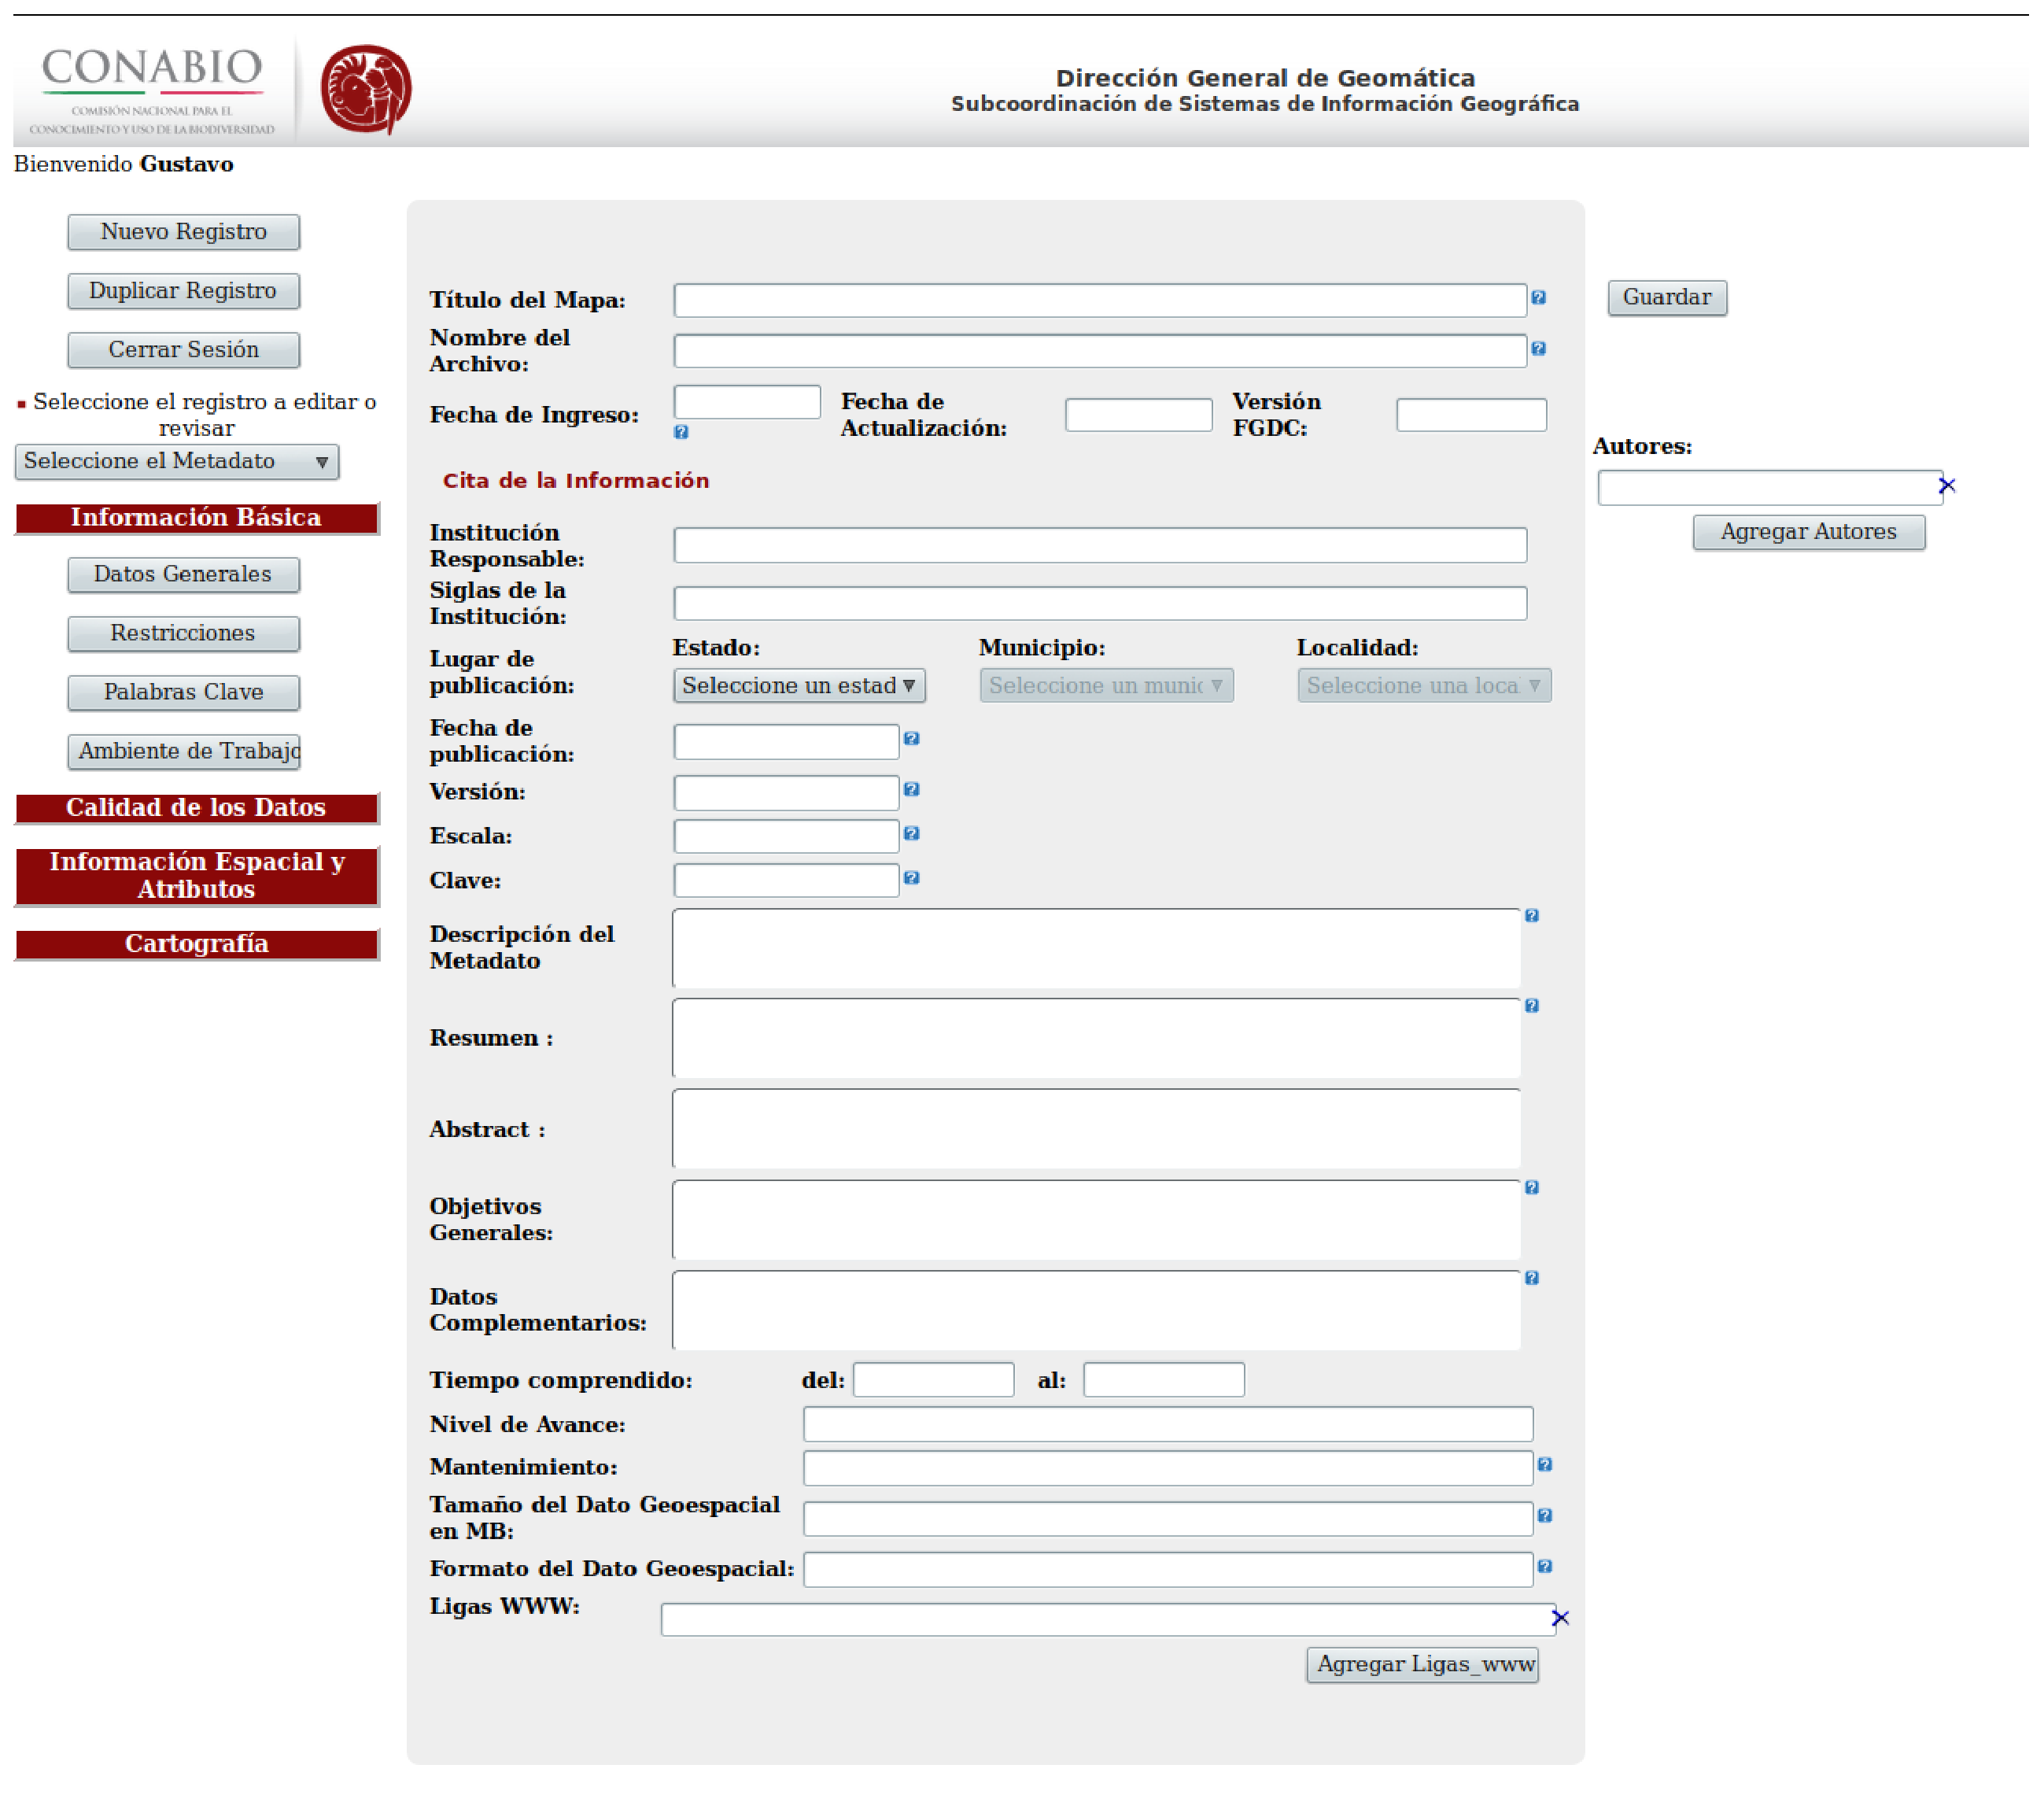
\includegraphics[width=12cm, height=12.5cm]{img/datosGenerales} %	
	\caption{Interfaz de Información básica}
\end{figure}


\section{Restricciones}
\subsection{Acceso}
\noindent{Restricciones y prerrequisitos legales de acceso al dato geoespacial, definidos por el productor. Puede tener uno de los siguientes datos: con restricciones o sin restricciones. El primero significa que el dato o datos geoespaciales no serán publicados por la CONABIO en su portal de geoinformación, en el caso de tratarse de cartografía generada a partir de un proyecto apoyado por la CONABIO, esta se publica una vez vencida la fecha de restricción acordada con la institución.}

\subsection{Uso}
\noindent{Restricciones y prerrequisitos legales de uso del dato geoespacial, puede ser: con restricciones o sin restricciones, conforme lo determine el autor del dato. Aunque haya restricciones de uso, eso no significa que dentro de la CONABIO no se puedan usar en determinados análisis o trabajos internos, aunque la CONABIO no podrá publicar el dato geoespacial.}

Es importante señalar que los valores de estos dos últimos campos están de acuerdo con las políticas de distribución de información de la CONABIO.

\subsection{Observaciones}
\noindent{Es el campo en el cual se puede agregar información adicional.}



\begin{figure}[h] %	
	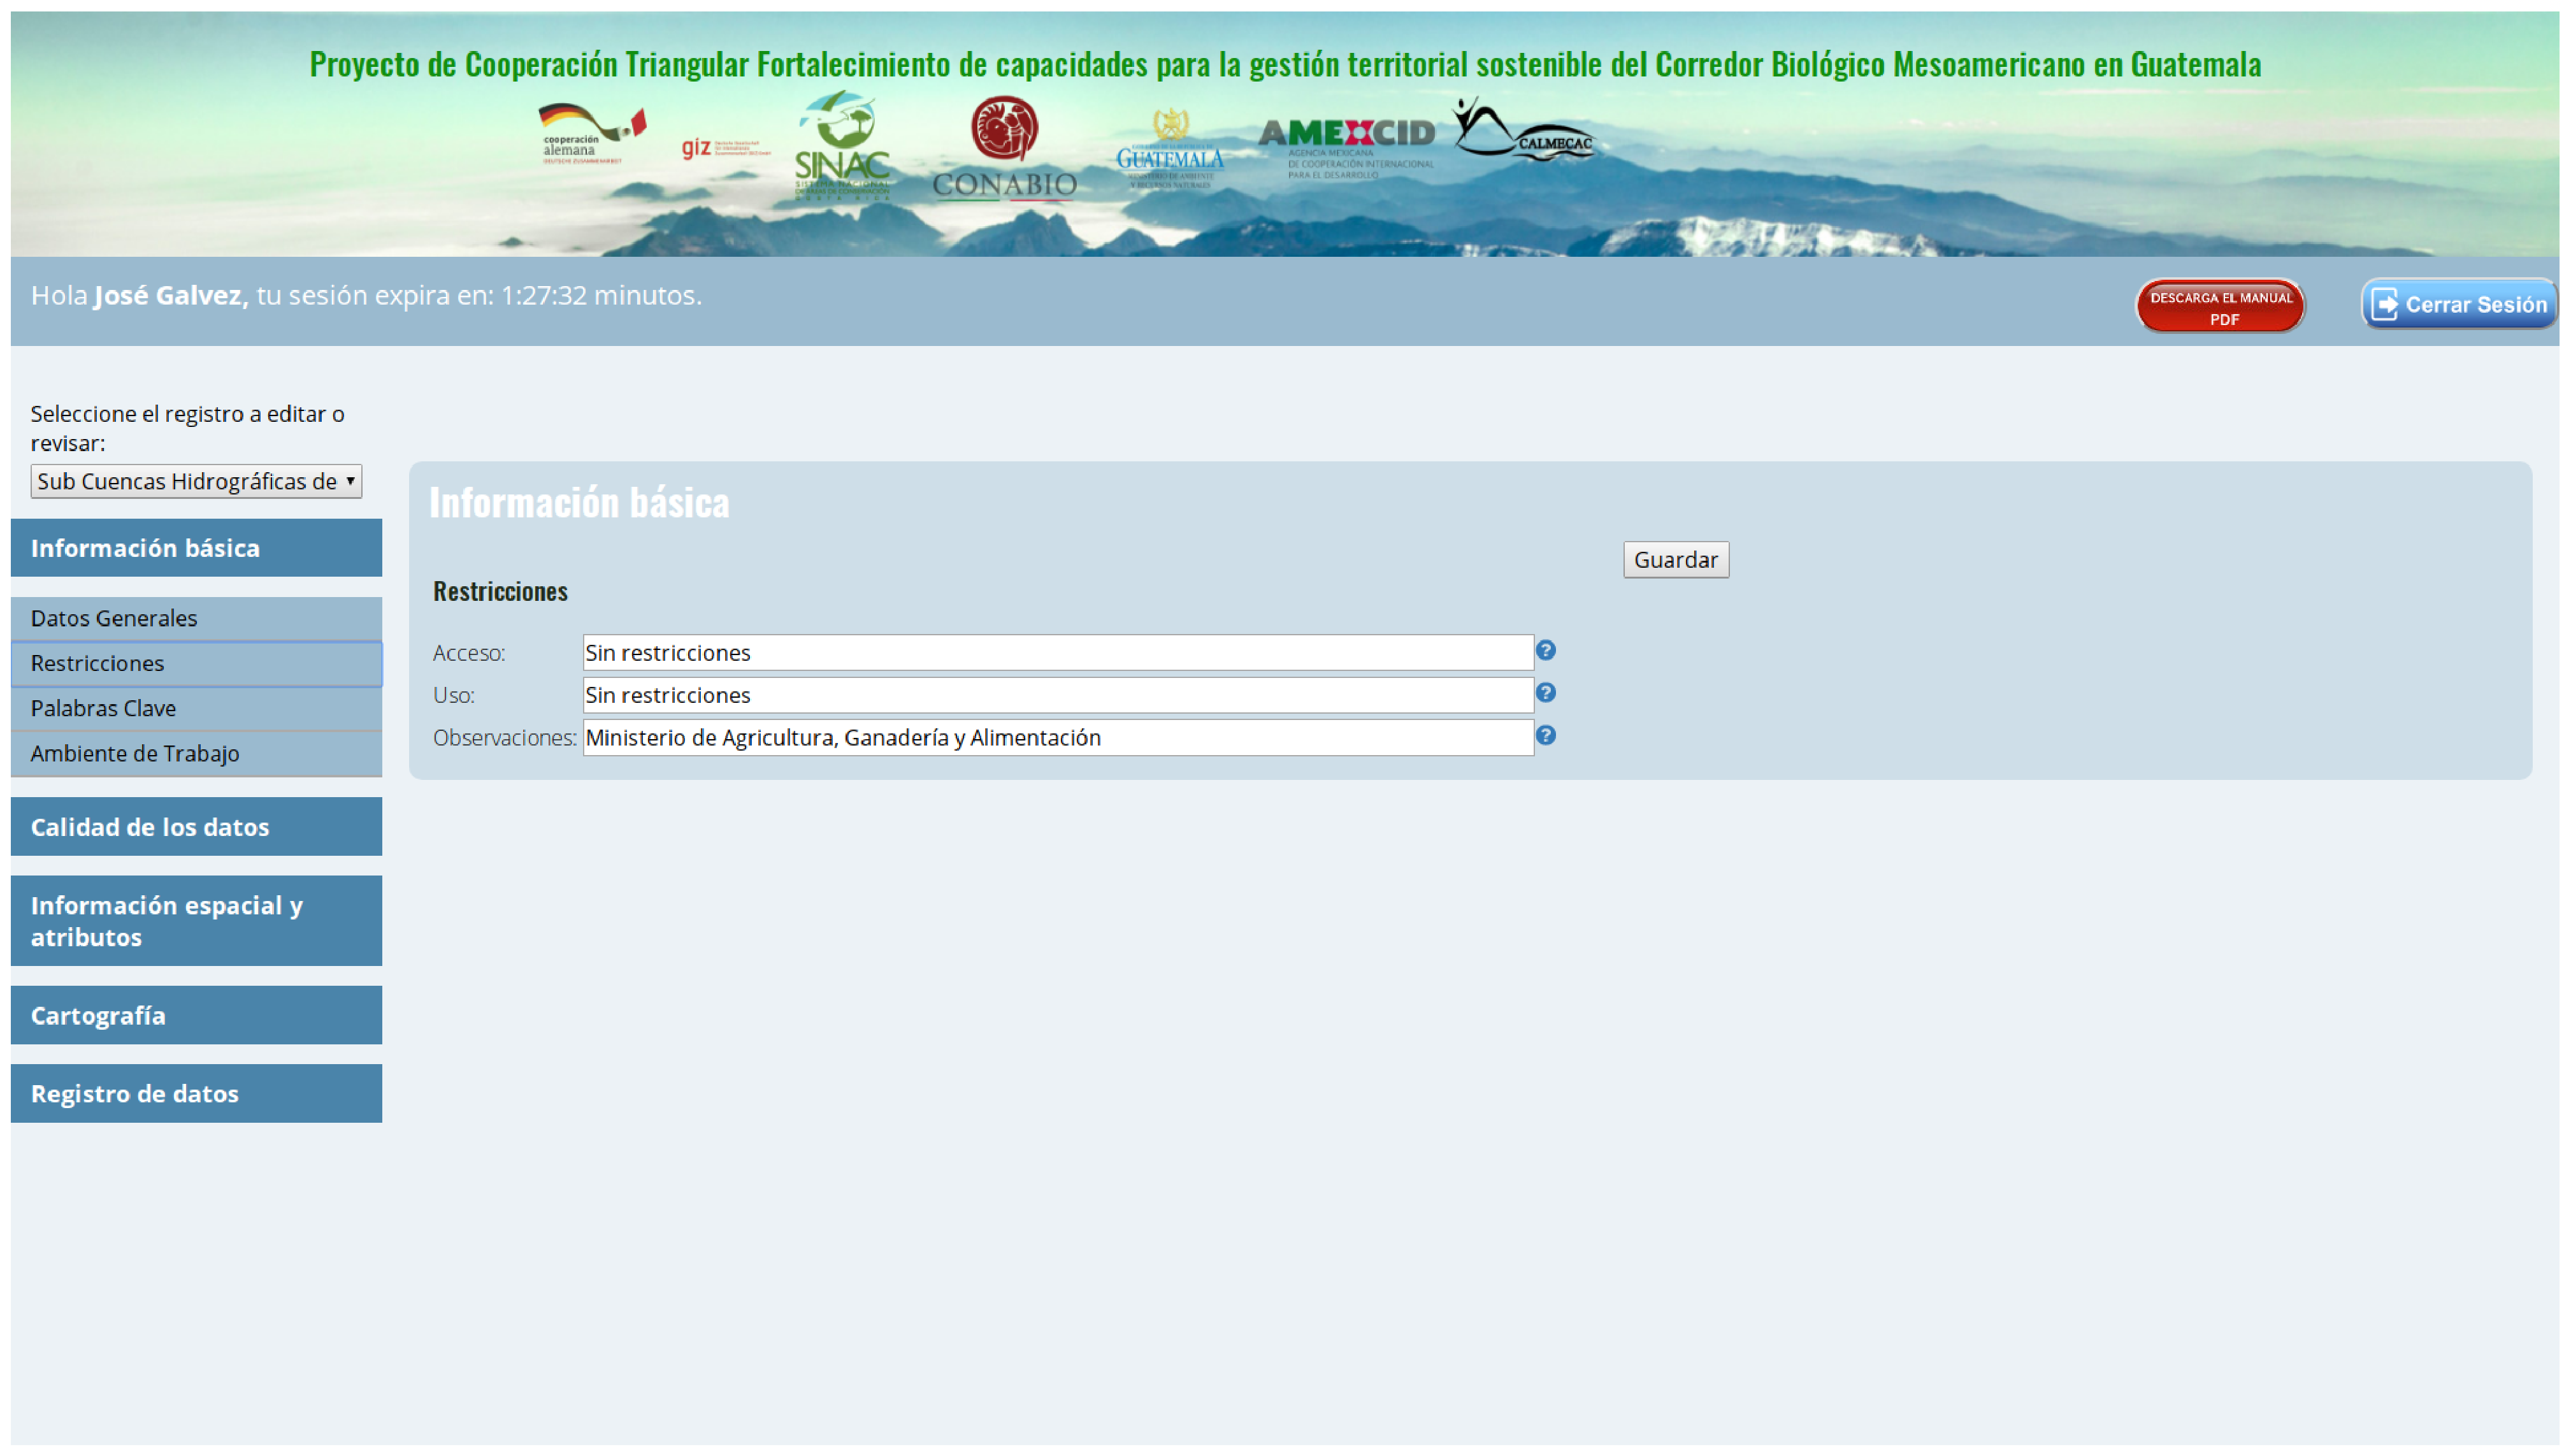
\includegraphics[width=12cm, height=6cm]{img/restricciones} %	
	\caption{Interfaz de Restricciones}
\end{figure}




\section{Palabras Clave}
\subsection{Temas}
\noindent{Palabras o frases, en forma de lista, que indican el significado o idea principal del tema del dato geoespacial, con el objetivo de que funcionen como palabras claves. Por ejemplo, humedal, vegetación, distribución potencial, mamíferos, etcétera. Como palabras obligatorias, deben agregarse los datos de escala, año y clave del proyecto (si aplica), sin que esto signifique que sean las únicas.}

No se permite el uso de caracteres alfanuméricos (metacaracteres). Por ejemplo: $@, ?, "", '$. Existen palabras o frases ya capturadas, sólo debe seleccionarlas a través del botón que se ubica al inicio de cada renglón de la lista.

\subsection{Sitios}
\noindent{Se listan nombres de lugares, municipios, entidades federativas, rasgos geográficos, regiones, etcétera, que aluden a la distribución geográfica del dato geoespacial (Área geográfica): por ejemplo, República Mexicana, Sierra Madre del Sur, Oaxaca, Reserva de la Biosfera Mariposa Monarca, etc.}

\section{Ambiente de Trabajo}
\noindent{Los siguientes campos son datos que corresponden al programa, equipo de cómputo y sistema operativo sobre el cual se elaboró el dato geoespacial. Los datos pueden cambiar en función de la actualización del equipo.}

\subsection{Software y hardware}
\noindent{Nombre del o los programa(s) de cómputo utilizado(s), incluyendo versión, y equipo de cómputo empleado para la elaboración del dato geoespacial. Por ejemplo, ArcMap ArcGIS ver. 10.1 y Dell Precision T5500.}

\subsection{Sistema Operativo}
\noindent{Nombre y versión del sistema operativo instalado en el equipo de computo empleado.}

\subsection{Requisitos técnicos}
\noindent{Especificaciones de software y hardware requerido para utiliza el dato, si es necesario.}

\subsection{Ruta y nombre de Archivo}
\noindent{Ruta y nombre del archivo}



\begin{figure}[h] %	
	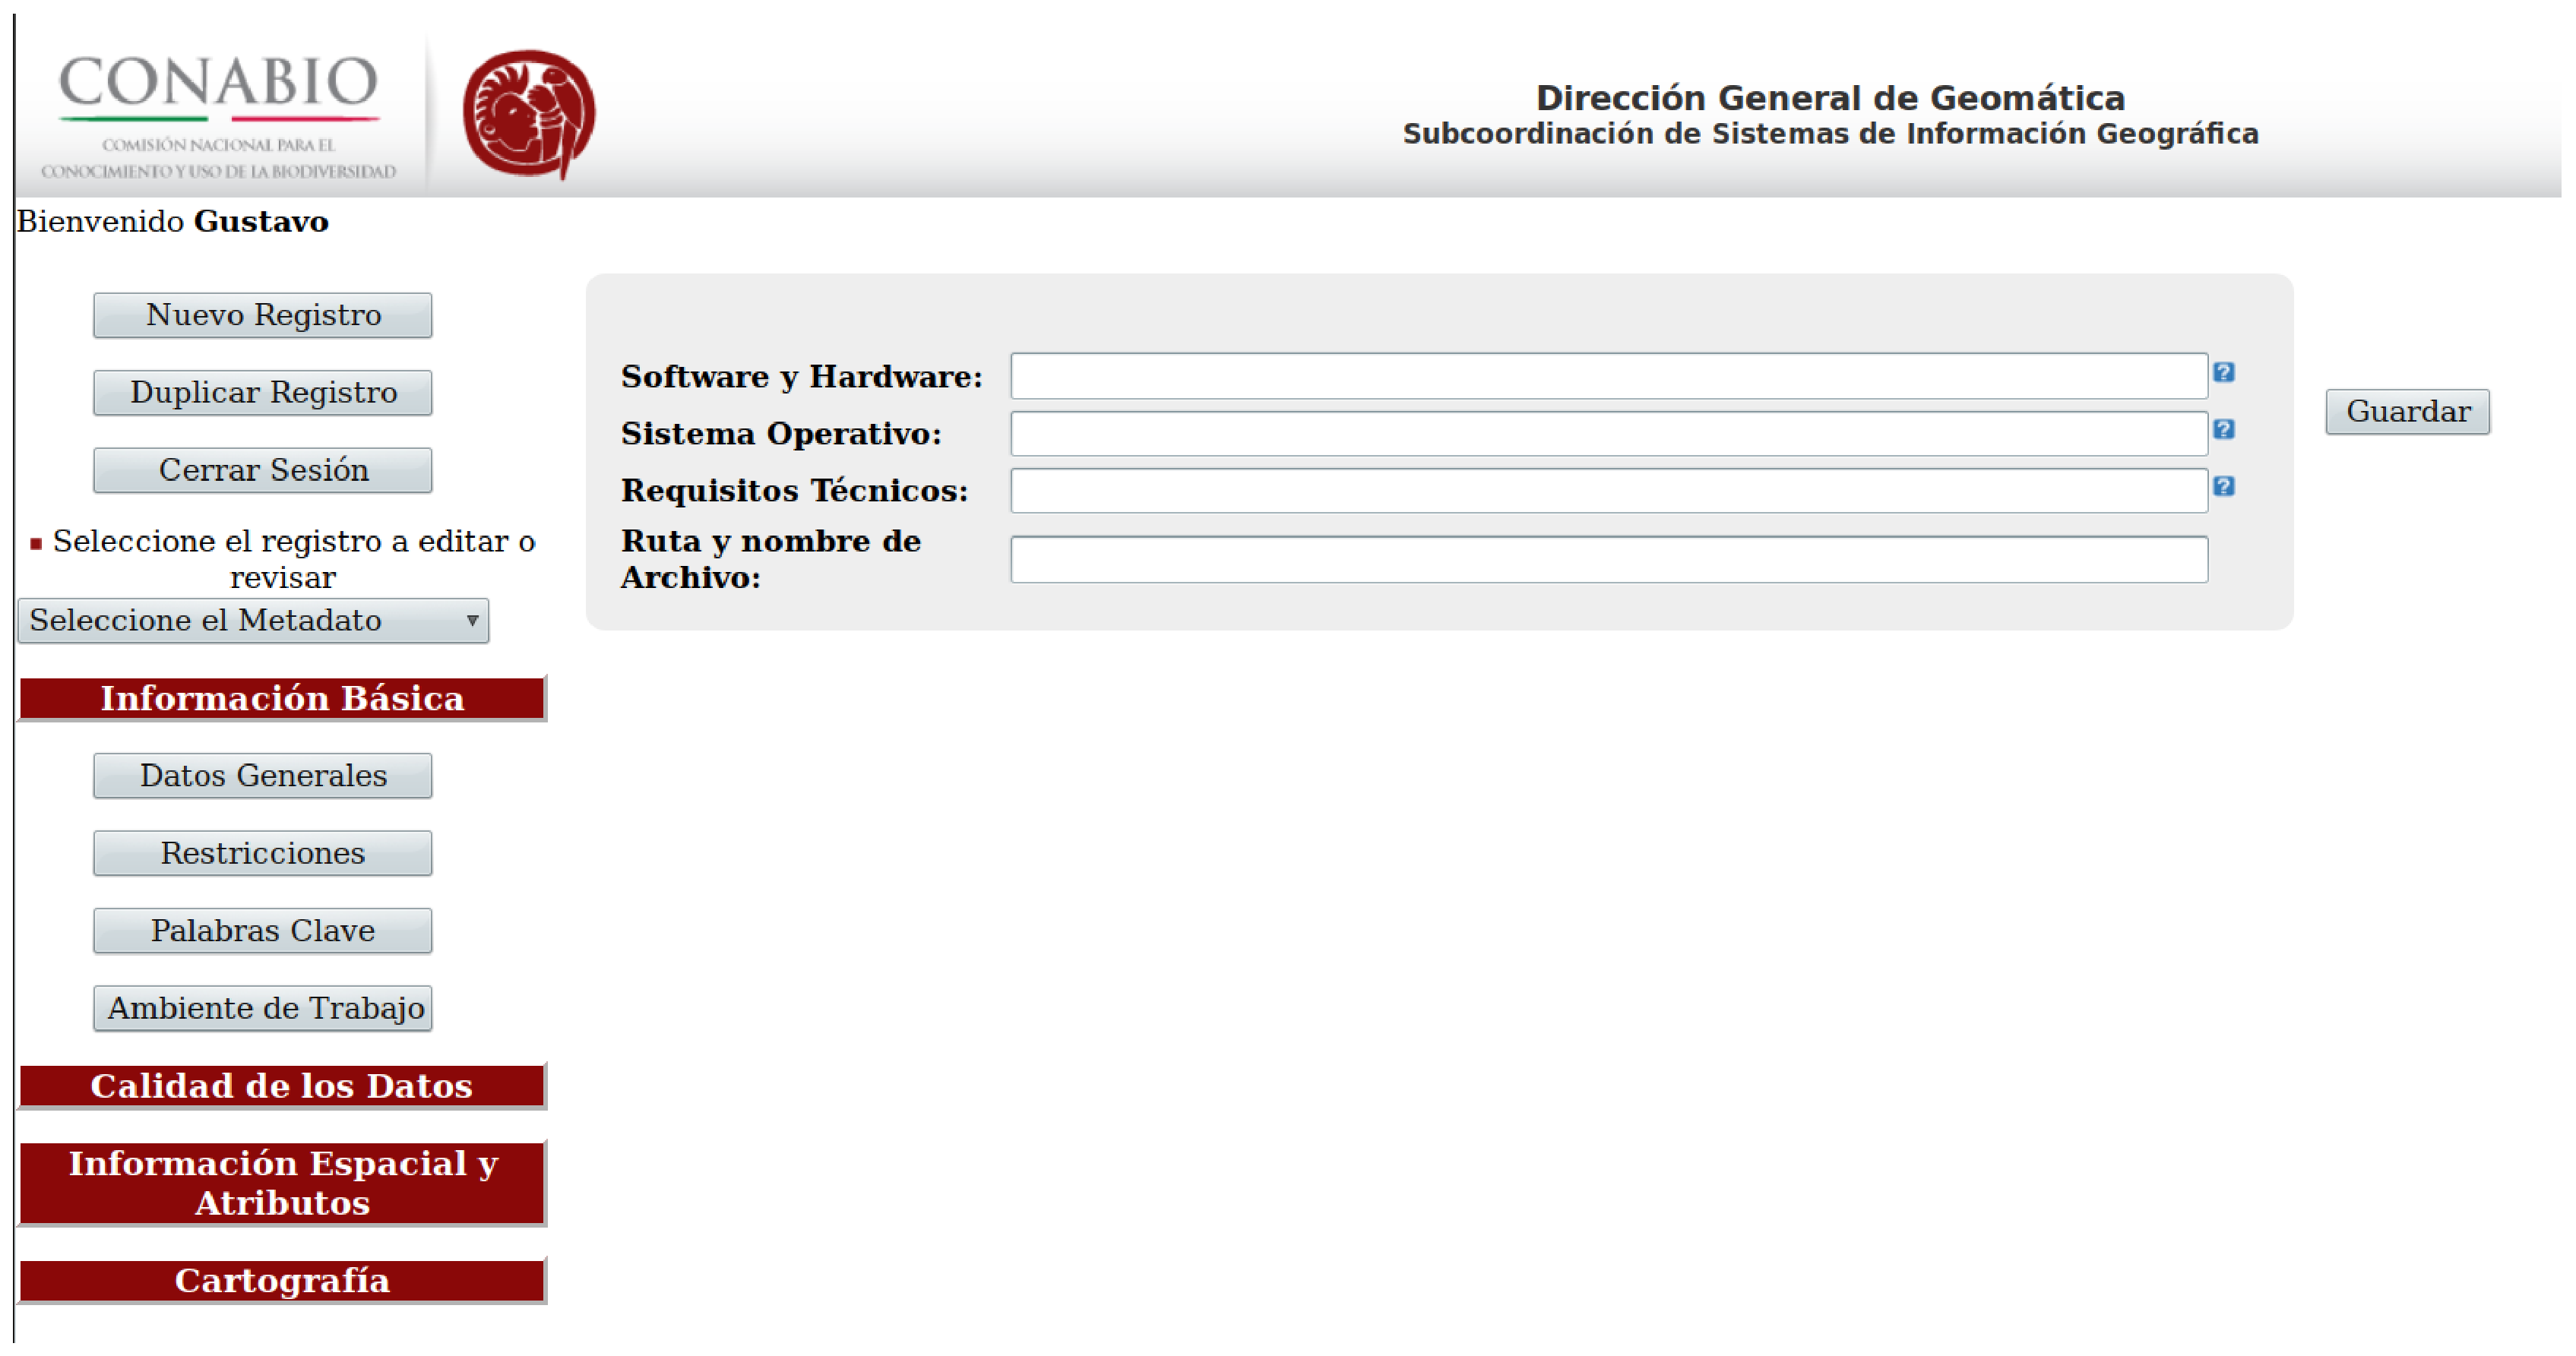
\includegraphics[width=12cm, height=6cm]{img/software} %	
	\caption{Interfaz de Ambiente de Trabajo}
\end{figure}









\chapter{Calidad de los datos}
\noindent{En esta sección se proporciona información detallada sobre la forma de elaboración del dato geoespacial, explicando la metodología usada, el proceso empleado, las referencias de la información utilizadas como insumo para obtener el dato geoespacial y datos taxonómicos si aplican.}

La sección se divide en dos partes: Calidad de los datos y Taxonomía.

A continuación se describen cada uno de los elementos compuestos y sus campos que forman parte de esta sección. Es importante que la captura se haga en el orden que se listan los campos.
\section{Calidad de los datos}
\subsection{Metodología}
\noindent{Señala el tipo de investigación según el lugar de aplicación para obtener o generar los datos que dieron origen el dato geoespacial. Puede ser: gabinete, campo, laboratorio, campo y gabinete, o campo, laboratorio y gabinete.}

\subsection{Descripción de la metodología}
\noindent{Se describe, de manera general, el o los métodos empleados en el proceso de elaboración del dato geoespacial, es decir, qué se hizo.}

\subsection{Descripción del proceso}
\noindent{Se describe ampliamente cómo se hizo el dato geoespacial, explicando lo realizado en cada uno de los métodos empleados, es decir, las actividades, técnicas y programas utilizados para generarlo.}

\section{Referencia de los datos originales}
\noindent{Se refiere al o los datos de referencia utilizados para la generación del dato geoespacial, que pueden ser datos georreferenciados en gabinete o campo, datos geoespaciales obtenidos de algún acervo, datos derivados de imágenes de satélite, etcétera. Estos pueden ser impresos o digitales. La referencia de cada dato utilizado deberá ser capturada en un atributo compuesto por separado. Por lo tanto, si para la elaboración del dato geoespacial se utilizaron dos capas en formato digital y un archivo de datos tabulares, se deberán capturar en forma de lista la referencia de dichos datos.}

\subsection{Título del Dato}
\noindent{Nombre del dato de referencia que fue usado como insumo para la elaboración del dato geoespacial.}

\subsection{Institución Responsable }
\noindent{Nombre de la Institución a la cual pertenece el dato de referencia.}

\subsection{Siglas de la Institución}
\noindent{Siglas de la Institución responsable del dato de referencia.}

\subsection{Lugar de Publicación}
\noindent{Lugar donde se publica el dato de referencia.}

\subsection{Versión}
\noindent{Edición del dato geoespacial o base de datos de referencia.}

\subsection{Escala}
\noindent{Escala del dato de referencia.}

\subsection{Fecha de Publicación}
\noindent{Fecha de publicación del dato de referencia.}

\subsection{Formato de Dato Geoespacial}
\noindent{Formato del dato de referencia, puede ser: impreso, digital, etc.}

\subsection{Tipo de Dato geoespacial}
\noindent{Indicar en qué formato se encuentra el dato de referencia.}

\subsection{Información}
\noindent{Se pide agregar que dato se obtuvo de esa información de referencia.}

\subsection{Otros}
\noindent{En esta sección se puede agregar cualquier información referente al dato de referencia.}

\subsection{Links}
\noindent{Se puede colocar citas de internet para complementar la información de referencia.}

\subsection{Autores}
\noindent{Nombre del autor o de los autores del dato de referencia. Tomando en cuenta la siguiente estructura; para el primer autor: apellidos seguido de coma, iniciales del o los nombres seguido de un punto; si el autor es una institución sólo se anota la sigla o acrónimo y segundo y tercer autor: inicial del o los nombres seguido de un punto; apellidos seguido de una coma.}

\section{Taxonomía}
\noindent{En el caso de que los datos geoespaciales representen la distribución de una o varias especies, deberá proporcionarse información taxonómica técnica o general de cada una de las especies que incluya el mapa.}

\textbf{Nota: No se pueden quedar jerarquías superiores vacías si se tiene una jerarquía inferior.}

\subsection{Cobertura General}
\noindent{En el caso de que no se conozca la información taxonómica técnica, puede usarse el nombre genérico por el cual se le conoce a la o las especies involucradas. Por ejemplo, aves, mamíferos, murciélagos, cactus, orquídeas, pastos, peces, etc.}

\subsection{Reino}
\noindent{Nombre del Reino al que pertenece la o las especies involucradas.}
\subsection{División o fila}
\noindent{Nombre de la División o Fila a la que pertenece la o las especies involucradas, según sea el caso.}
\subsection{Clase}
\noindent{Nombre de la Clase a la que pertenecen la o las especies en cuestión.}
\subsection{Familia}
\noindent{Nombre de la Familia a la que pertenecen la o las especies involucradas.}
\subsection{Género}
\noindent{Nombre del Género al que pertenece la o las especies tratadas.}
\subsection{Especie}
\noindent{Nombre científico de la especie involucrada (género y epíteto específico).}
\subsection{Nombre común}
\noindent{Nombre vulgar o común por el cual se le conoce a la especie. Si es más de un nombre, separarlos por comas.}

\subsection{Cita}
\noindent{Cita de la publicación o publicaciones en las que se basa el sistema de clasificación taxonómica. No se permite el uso de metacaracteres (ejemplo: @, ?, "", ').}

\subsection{Título}
\noindent{Nombre del libro, revista, etc. que fue utilizado en el proyecto para la obtención de la información taxonómica.}

\subsection{Institución}
\noindent{Nombre de la Institución a la cual pertenece el dato de referencia.}

\subsection{Siglas}
\noindent{Siglas de la Institución responsable del dato utilizado.}

\subsection{Lugar}
\noindent{Ciudad o lugar donde se llevo a cabo la publicación.}

\subsection{Versión}
\noindent{Es sinónimo de edición.}

\subsection{Fecha}
\noindent{Corresponde a la fecha de publicación del dato utilizado.}

\subsection{Clave}
\noindent{Corresponde a la clave del proyecto asignada por la CONABIO, si aplica.}

\subsection{Descripción}
\noindent{Es un campo donde se aporta información complementaria a la cita de la referencia taxonómica.}

\subsection{Autores}
\noindent{Nombre del autor o de los autores del dato utilizado. Tomando en cuenta la siguiente estructura; para el primer autor: apellidos seguido de coma, iniciales del o los nombres seguido de un punto; si el autor es una institución sólo se anota la sigla o acrónimo y segundo y tercer autor: inicial del o los nombres seguido de un punto; apellidos seguido de una coma.}

\begin{figure}[h] %	
	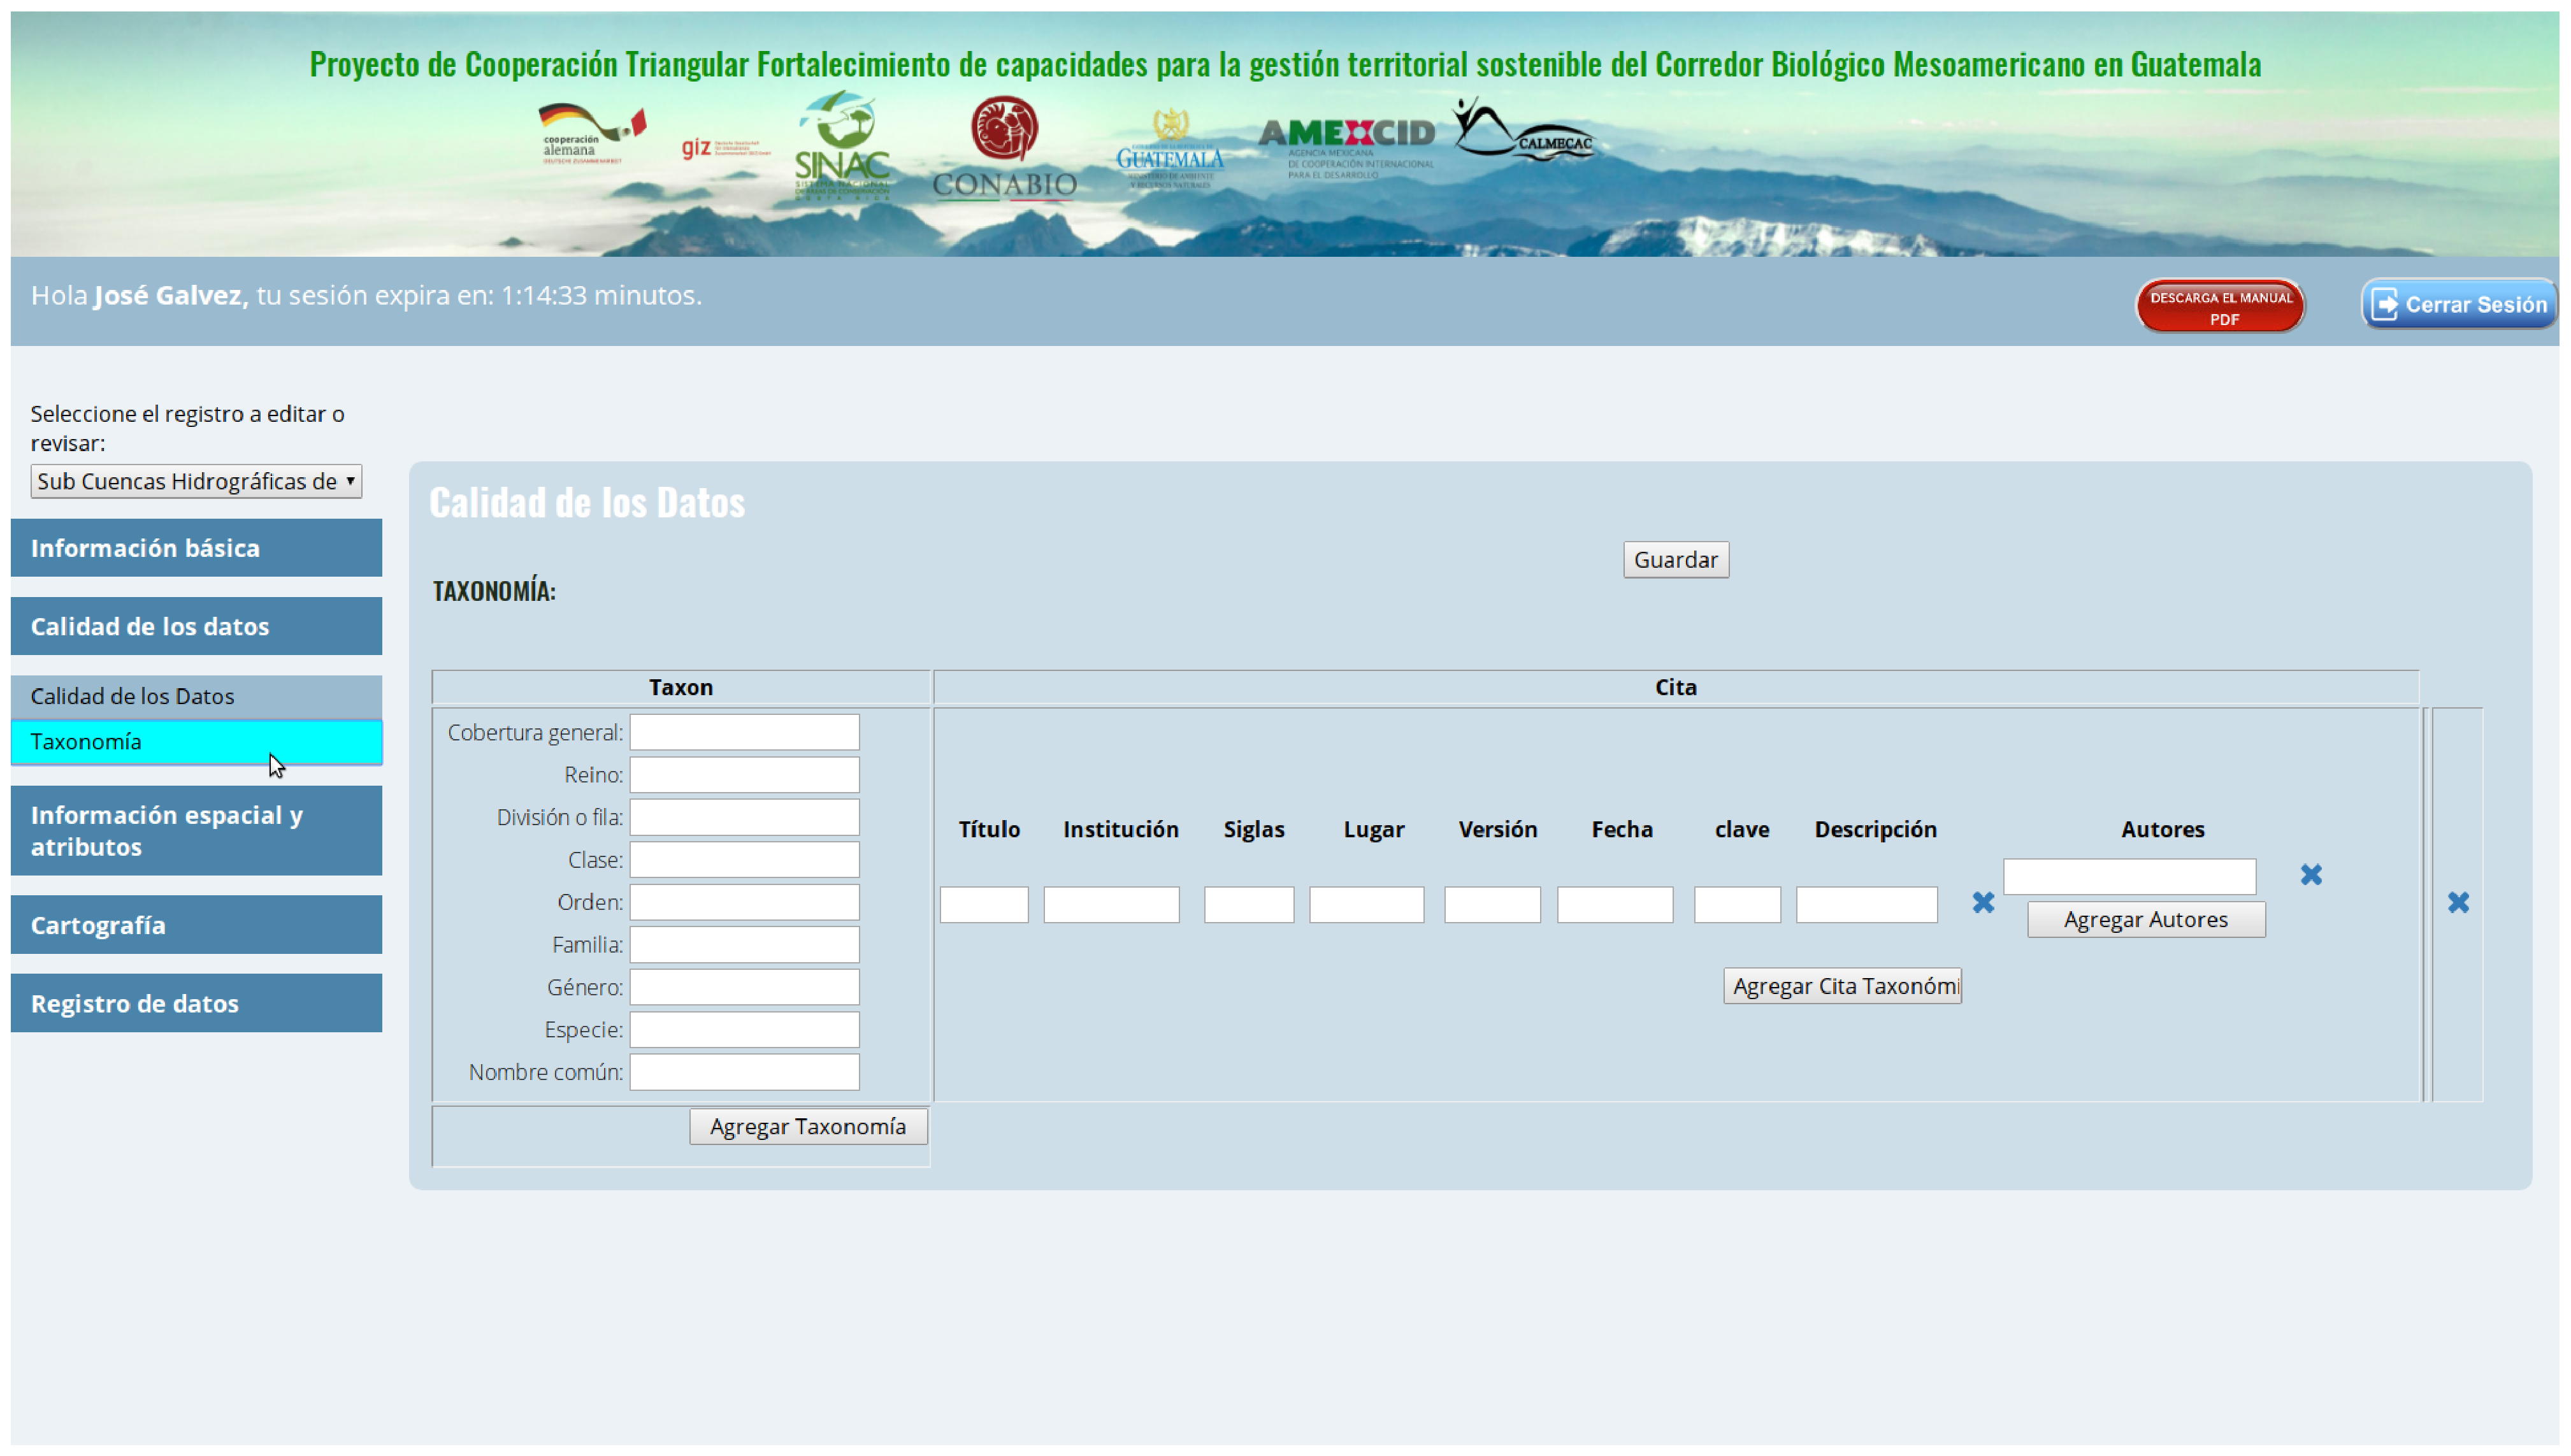
\includegraphics[width=12cm, height=4cm]{img/taxonomia} %	
	\caption{Interfaz de Taxonomia}
\end{figure}

\chapter{Información Espacial y Atributos}
\noindent{En esta sección se proporciona información detallada sobre el dato geoespacial. Describiendo su geometría, representación espacial, proyección cartográfica y las características que califican y describen el dato.}

La sección se divide en tres partes o elementos compuestos que son: Datos espaciales, Proyección cartográfica y Atributos.

A continuación se describen cada uno de los elementos compuestos y sus campos. Es importante que la captura se haga en el orden que se enlistan los campos.

\section{Información Espacial}

\subsection{Estructura del Dato}
Se especifica la estructura del dato geoespacial seleccionando una de las siguientes opciones: Vector o Raster.

\subsection{Tipo del dato}
\noindent{Es el tipo de representación (geometría) de los objetos del mundo real a través de los datos geoespaciales. El dato puede estar representado por: puntos, líneas y polígonos (si la estructura es vectorial); y píxel (si la estructura es raster).}

\subsection{Número total del Dato}
\noindent{Se escribe el número total de elementos que contiene el dato geoespacial si es vectorial, y si es raster se debe multiplicar las columnas por renglones.}

\section{Coordenadas del Extremo}
\noindent{Coordenadas extremas del área geográfica que ocupa el dato geoespacial (oeste, este, norte y sur) y definido por el programa utilizado para su elaboración. Los valores indican la extensión del dato sobre la superficie de la tierra mediante coordenadas geográficas (grados decimales). Ejemplo: Oeste: -117.12; Este: -103.08; Norte: 32.64; y Sur: 22.87.}

\section{Proyección Cartográfica}
\noindent{Para capturar esta la información se debe seleccionar de la tabla, la proyección del dato geoespacial. Las proyecciones enlistadas van de acuerdo con los lineamientos cartográficos (UTM, Cónica Conforme de Lambert o Coordenadas Geográficas).}

\subsection{Datum horizontal}
\noindent{WGS84, de acuerdo con los lineamientos cartográficos. }

\subsection{Nombre del elipsoide}
\noindent{WGS84, de acuerdo con los lineamientos cartográficos.}
\subsection{Área geográfica}
\noindent{Descripción textual breve de la distribución geográfica del dato geoespacial, ya sea ésta nacional, regional o local. Ejemplo: República Mexicana, Norte de Chihuahua, San Luis Potosí, etc.}

\section{Si la estructura es Raster}
\noindent{Es necesario proporcionar la siguiente información.}

\subsection{Número de renglones}
\noindent{Número total de renglones a lo largo del eje Y.}

\subsection{Número de columnas}
\noindent{Número total de columnas a lo largo del eje X.}

\subsection{Tamaño del píxel de X en metros}
\noindent{Resolución espacial, en metros, del píxel sobre el eje X.}

\subsection{Tamaño del píxel de Y en metros}
\noindent{Resolución espacial, en metros, del píxel sobre el eje Y. Es importante mencionar que para el tamaño del pixel en X y Y, el caso de que el dato geoespacial este referido a un sistema de coordenadas geográficas, el valor se obtiene multiplicando el tamaño del pixel en grados por un valor estándar aproximado en el Ecuador, en donde 1 grado = 111.111 km.}

\subsection{Coordenada X del origen del raster}
\noindent{Coordenada en grados decimales o en metros, según la proyección, del punto de origen del raster sobre el eje X, que corresponde a la esquina superior izquierda del raster.}

\subsection{Coordenada Y del origen del raster}
\noindent{Coordenada en grados decimales o en metros, según la proyección, del punto de origen del raster sobre el eje Y, que corresponde a la esquina superior izquierda del raster.}


\begin{figure}[h!] %	
	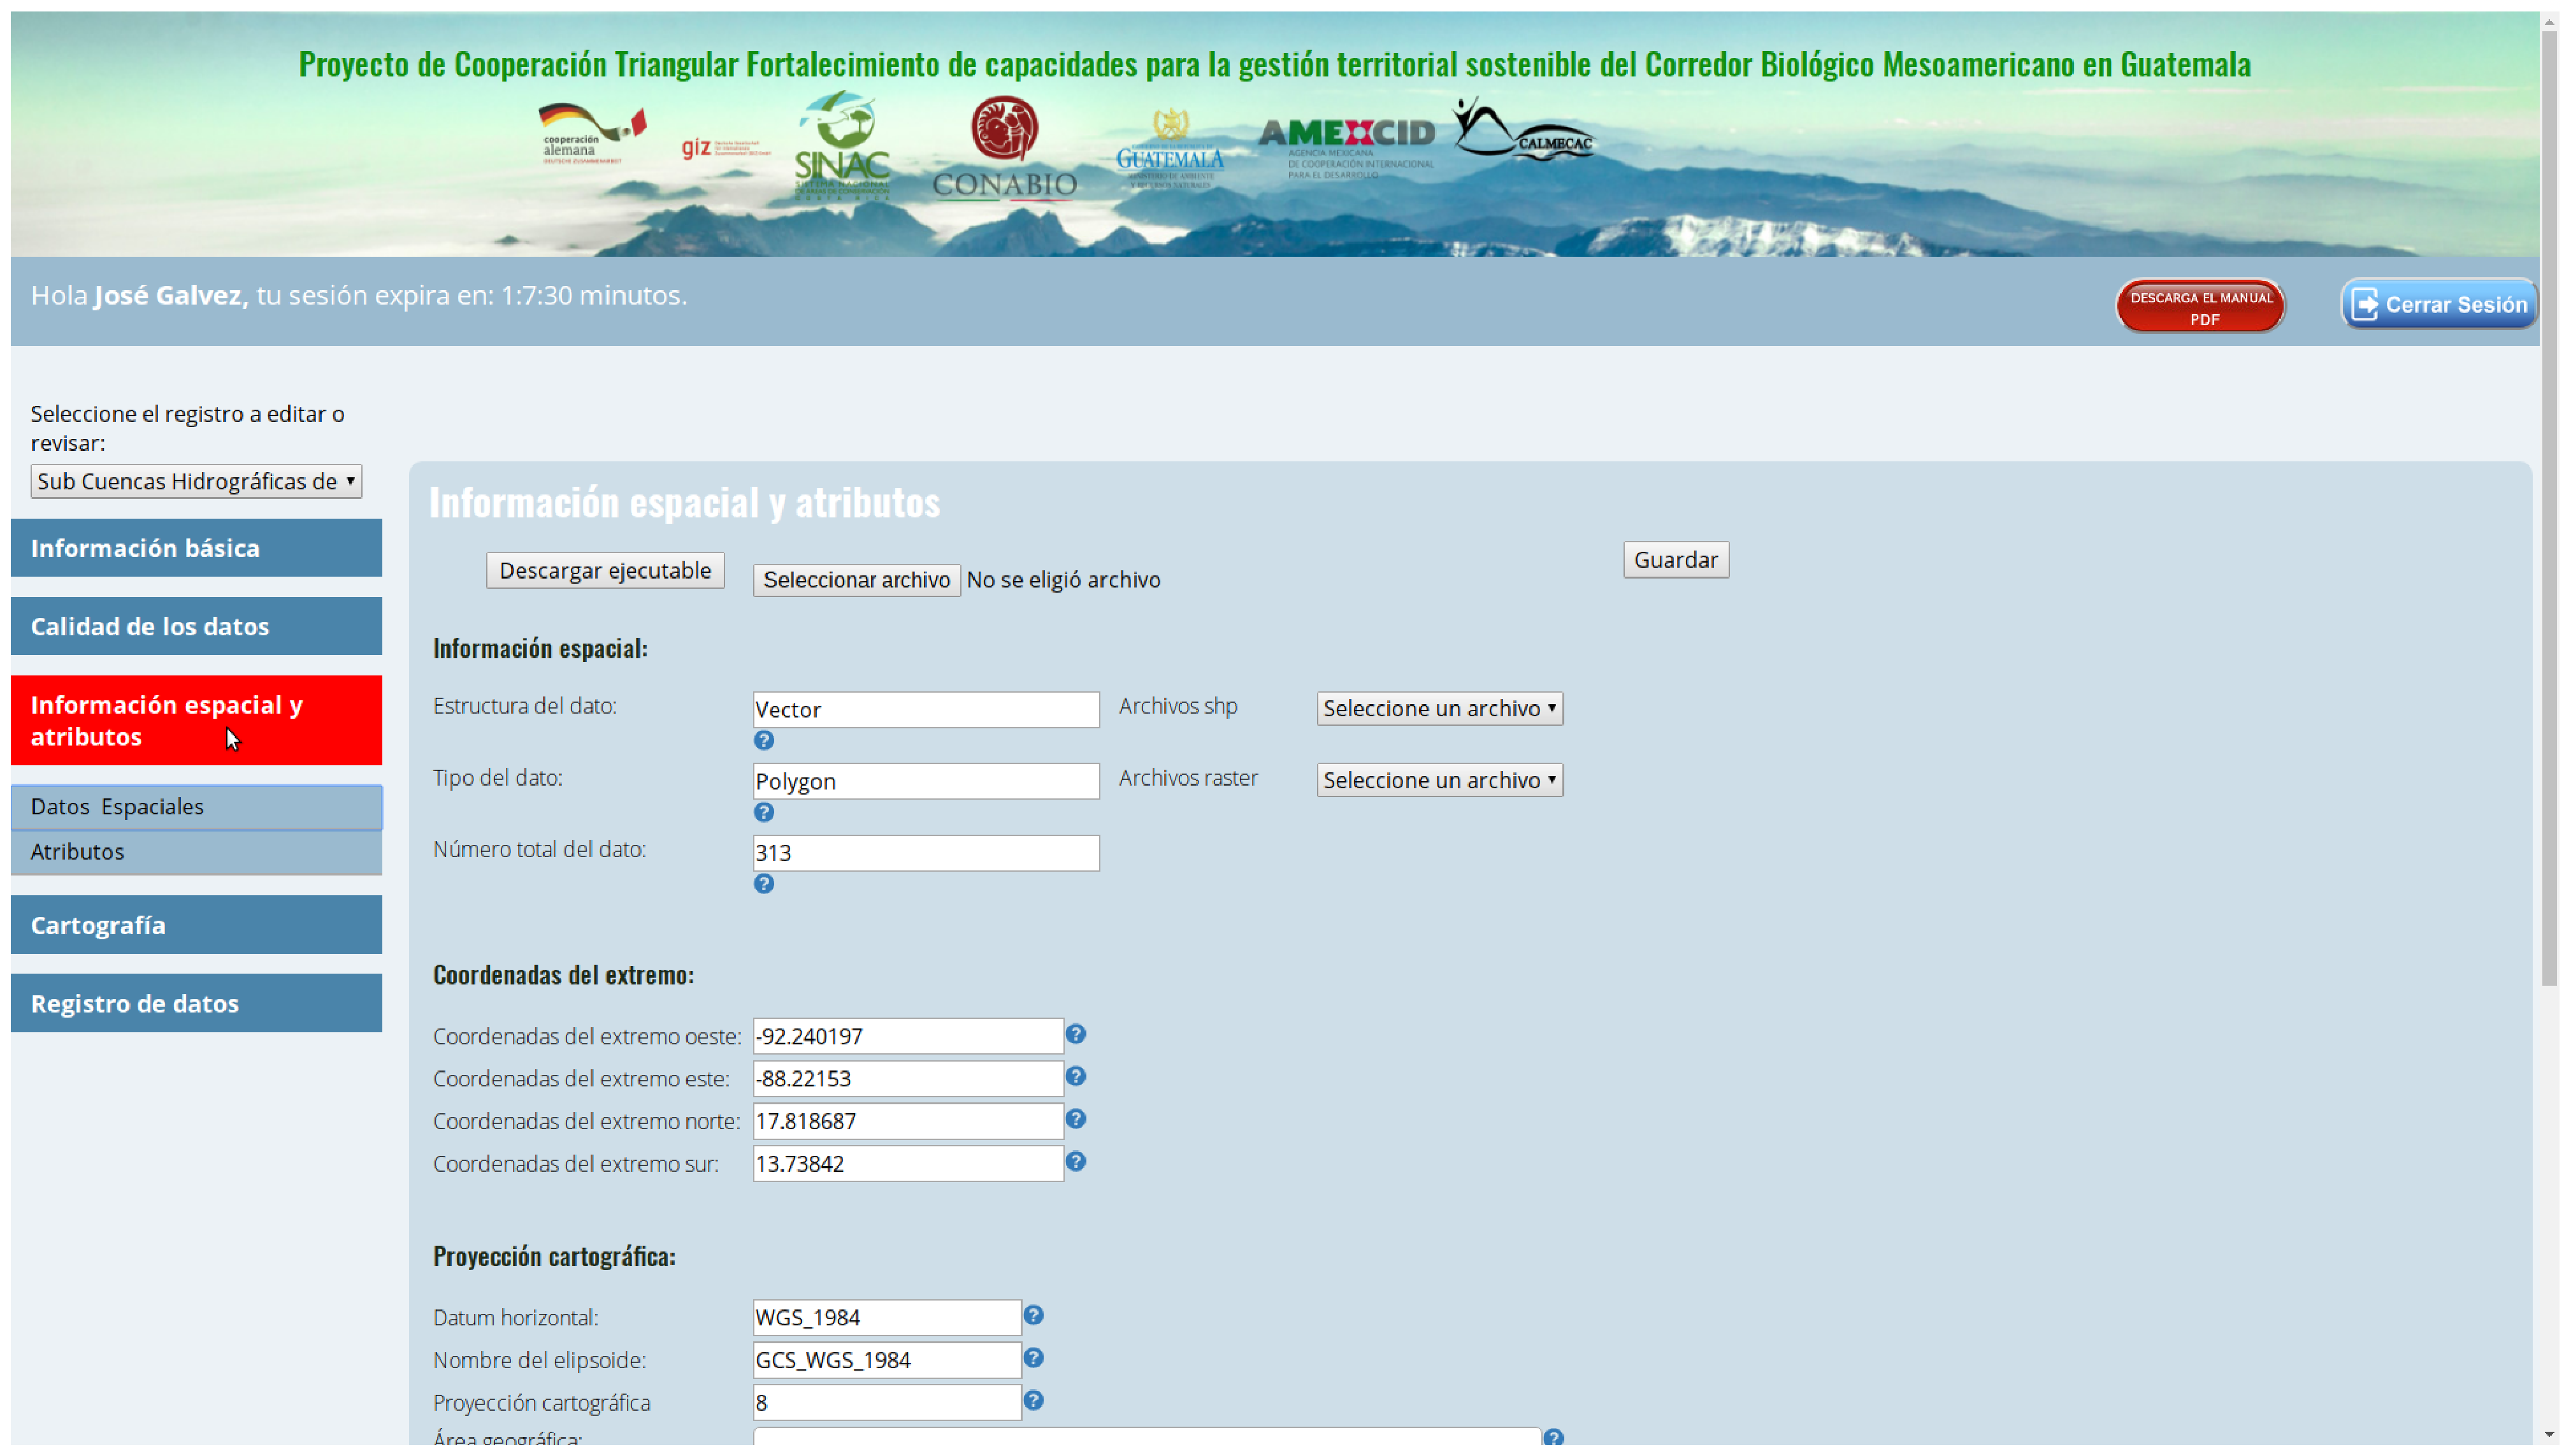
\includegraphics[width=12cm, height=13cm]{img/datosEspaciales} %	
	\caption{Interfaz de Datos Espaciales}
\end{figure}





\section{Atributos}
\noindent{Información obtenida a partir de la tabla del dato geoespacial.}

\subsection{Nombre de la Entidad (Tabla)}
\noindent{Nombre del archivo que contiene los atributos del dato geoespacial (capa digital). Si el dato geoespacial es un shapefile manejar el nombre del dato con extensión .dbf. (Y si el dato es de estructura raster, para un grid de Arc/Info manejar el nombre del dato con la extensión .vat).}

\subsection{Descripción de la Entidad (Tabla)}
\noindent{Descripción breve del contenido de la tabla del dato geoespacial. Los siguientes incisos describen los campos que contiene la tabla del dato geoespacial, por lo tanto se repetirán “n” veces dependiendo de cuantos campos tenga la tabla.}

\subsection{Nombre}
\noindent{Corresponde al nombre del campo que describe alguna característica o valor del dato geoespacial. Se deberá anotar tal cual como se muestra en el dato geoespacial.}

\subsection{Descripción}
\noindent{Breve descripción del contenido del atributo, que dependerá de la información que contenga el mismo.}

\subsection{Fuente}
\noindent{A través de qué o quién se definió el nombre, características y uso del atributo. Puede ser un software, responsable del proyecto, una institución, etc.}

\subsection{Unidades de medida}
\noindent{En qué unidades está definido el atributo. Pueden ser: metros, grados decimales, metros cuadrados, mm, grados centígrados, etc. Si el tipo de dato del atributo es carácter, entonces se deja vacío el campo. Se recomienda verificar la lista ya existente, utilizando el botón.}

\subsection{Tipo de dato}
\noindent{Corresponde al tipo de dato que representa los valores de un campo y puede ser de tipo carácter o numérico. Se recomienda verificar la lista ya existente, utilizando el botón.}

\begin{figure}[h!] %	
	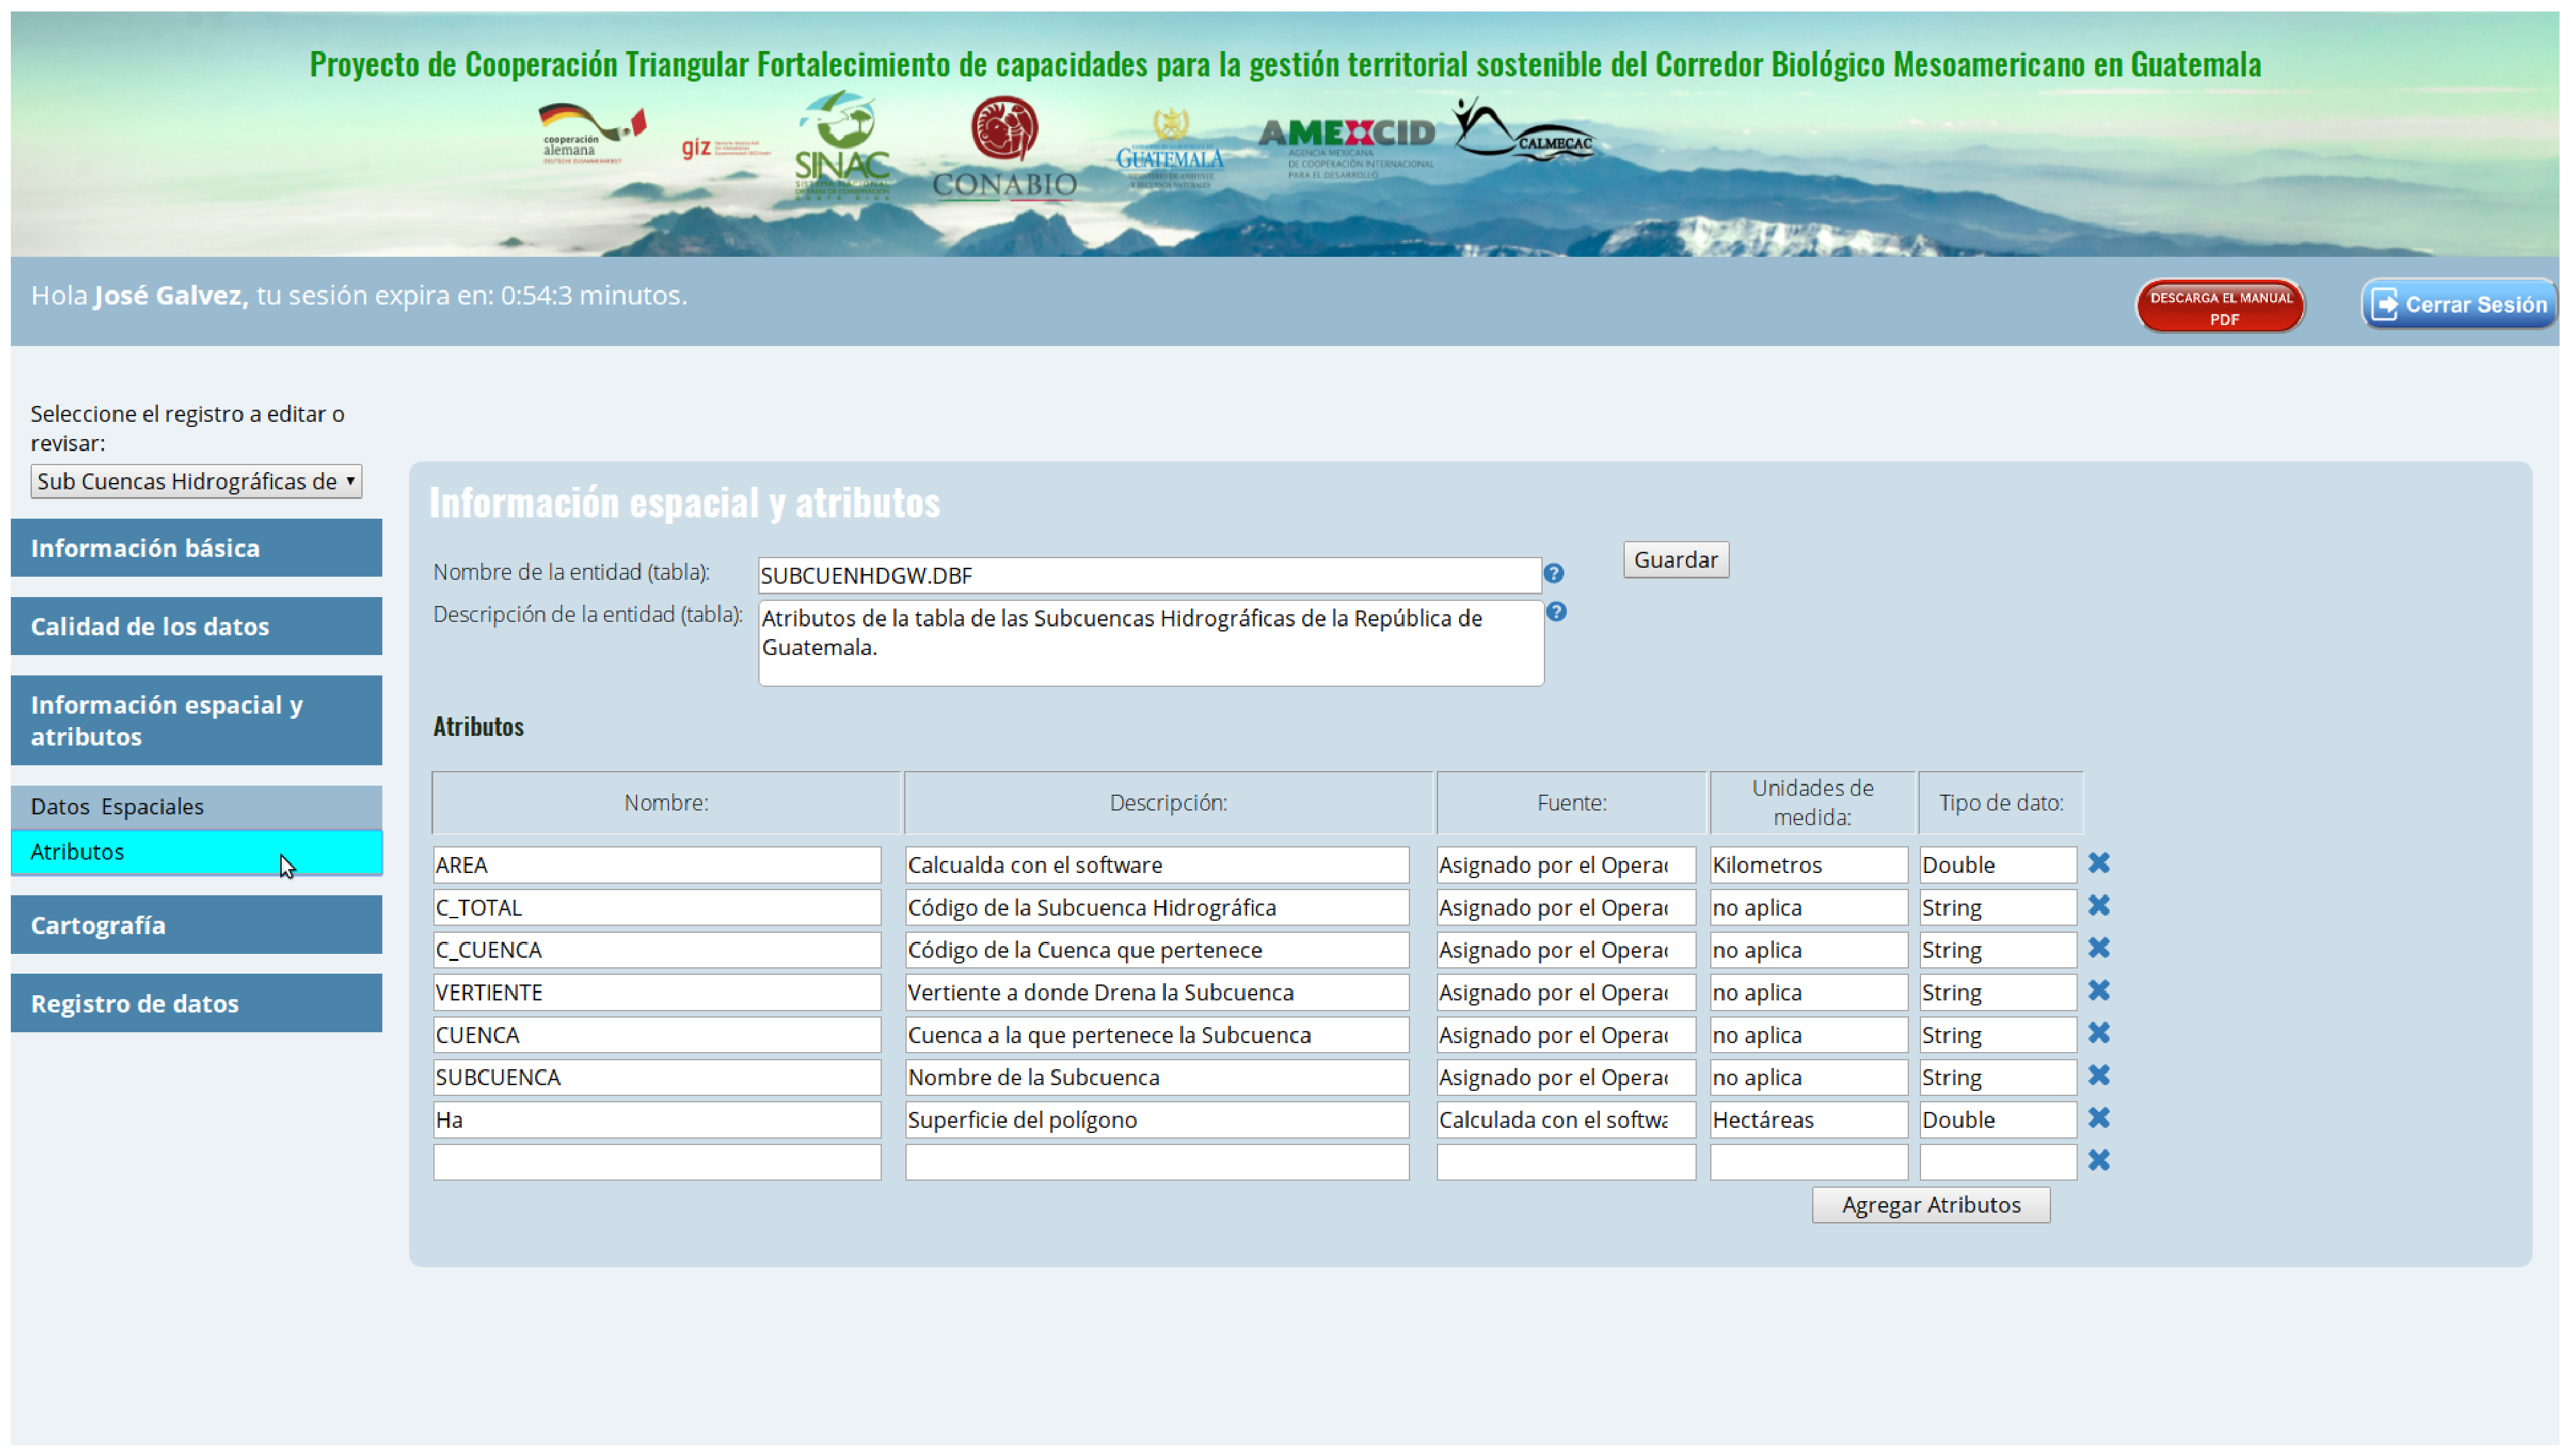
\includegraphics[width=12cm, height=4cm]{img/ambienteDeTrabajo} %	
	\caption{Interfaz de Atributos}
\end{figure}


\section{Cartografía}
\subsection{Subir archivos}

\noindent{Una vez capturados y guardados los metadatos, es posible enviar la cartografía correspondiente a la CONABIO para ser previsualizada en el geoportal de la CONABIO.}

Para esto, en esta sección aparece el botón con la leyenda Subir archivos. Si el archivo es el correcto se publicará la cartografía en un servidor de mapas (En este caso Geoserver) para su visualización.

Hay que tener en cuenta que para que sea posible la publicación del archivo se debe de cumplir que:
\begin{enumerate}
\item La cartografía debe de corresponder a los metadatos capturados, pues de no ser así, el archivo no podrá subir.

\item El archivo que se adjuntará para su publicación es con extención .zip y el cual contiene los cuatro archivos fundamentales con extenciones prj, shp, shx, y bdf.

\item Los cuatro archivos fundamentales deben de tener el mismo nombre que se asignó al nombre de archivo del metadato.

\item Aunque los servidores de la CONABIO están protejidos contra ataques informáticos, así como de malware, se pide que se verifique la integridad del archivo zip.

\end{enumerate}

\begin{figure}[h!] %	
	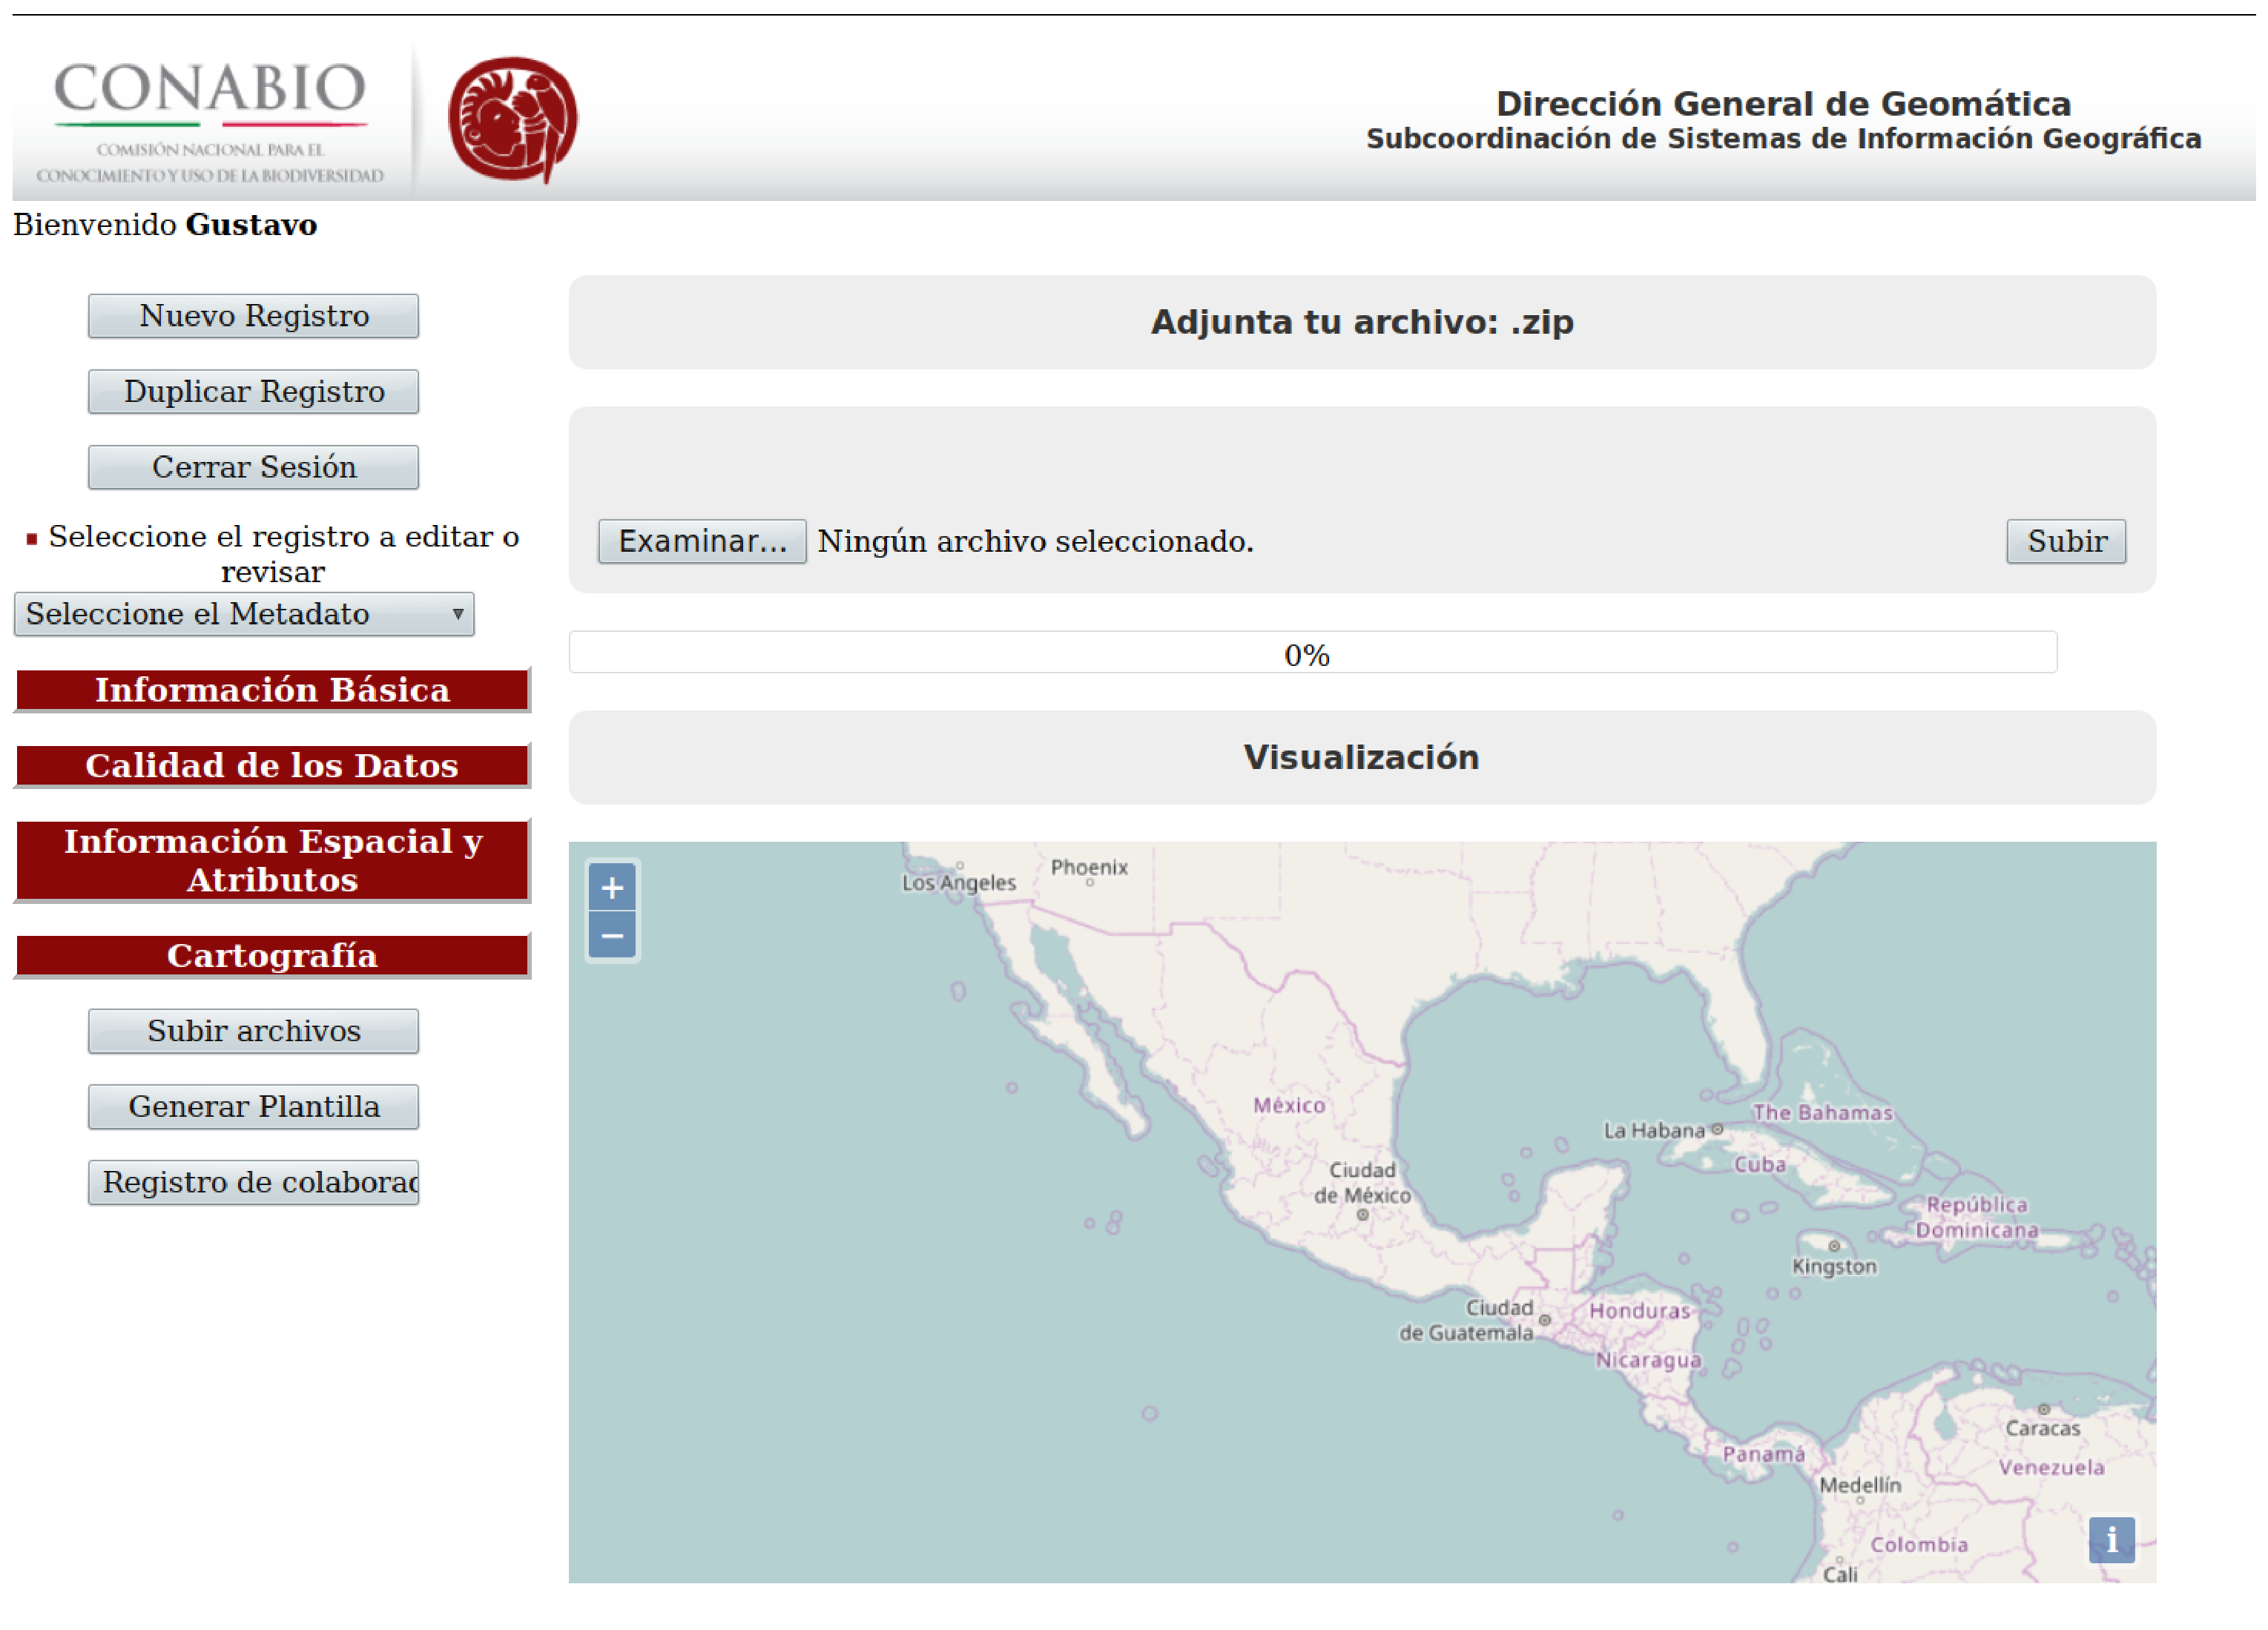
\includegraphics[width=12cm, height=8cm]{img/cartografiaCargaArchivos} %	
	\caption{Interfaz de Carga de Archivos}
\end{figure}
\section{Registro de colaboradores}

\noindent{Esta sección está dedicada a la alta y baja del personal que colabora en la plataforma de captura de metadatos. Para esto se han definido los siguientes roles de participación:}
\begin{enumerate}
\item Capturista
\item Analista (coordinador)
\item Administrador
\end{enumerate}

\textbf{Caturista}. Es aquella persona que ingresa los datos al módulo de información cartográfica, llena los formularios, y guarda la información. Este rol no puede subir cartografía al módulo.

\textbf{Analista}. Este rol es quien además de poder editar y validar la información, puede subir la cartografía al módulo. Por lo que es responsable de que la información que se captura sea correcta y de que lo que se sube a los servidores de CONABIO esté en perfecto estado topológico. Así como libre de malware. En este sentido, el analista puede tener uno o varios capturistas a su cargo, por lo que funge también como coordinador de ellos.

El analista puede dar de alta a uno o varios capturistas. Y es quien coordina el trabajo del equipo.   

\textbf{Administrador}. El aquel que puede dar de alta/baja a analistas como capturistas. Pero también puede dar de alta a otro administrador. Es quien está a cargo de que el sistema funcione correctamente y de atender todas aquellas contingencias que puedan ocurrir.

\begin{figure}[h!] %	
	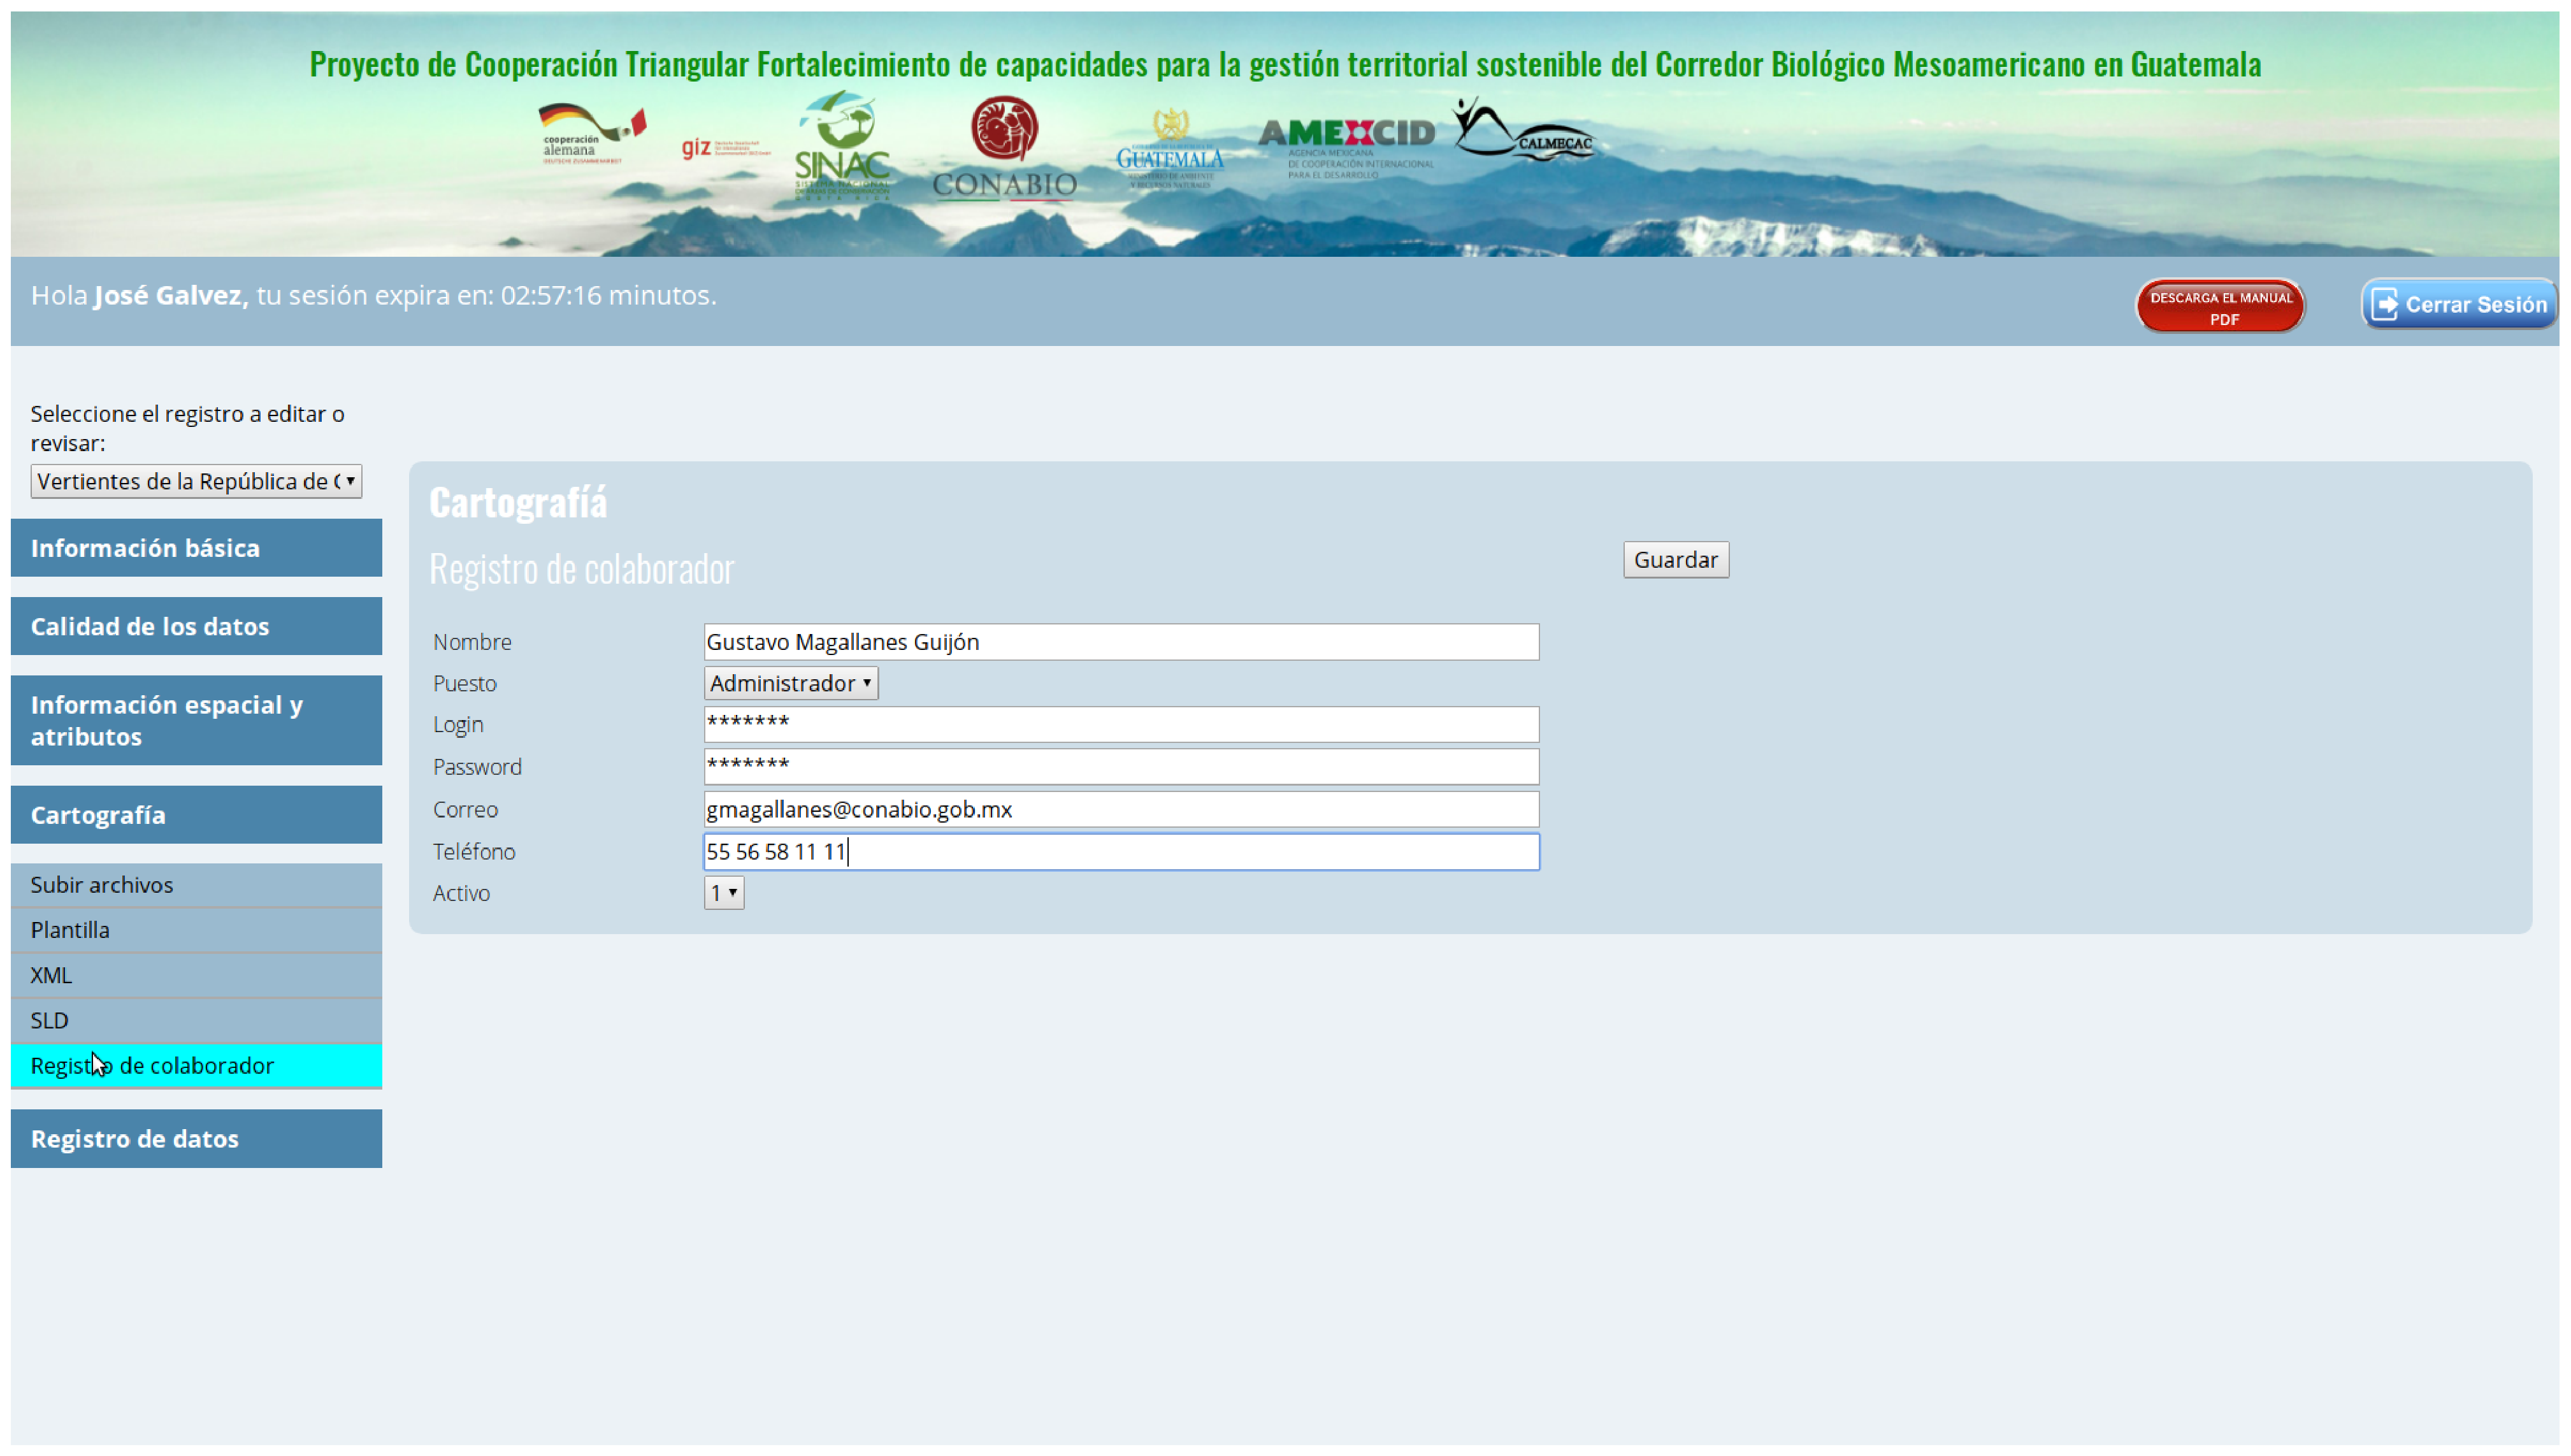
\includegraphics[width=12cm, height=6cm]{img/registroColaboradores} %	
	\caption{Interfaz de Registro de Colaboradores}
\end{figure}


\chapter*{Apendice. Ejemplos}
\addcontentsline{toc}{chapter}{Apendice. Ejemplos}
\section*{Ejemplo 1}
\section*{Poligonal y zonas núcleo y de amortiguamiento de la Reserva de la Biosfera Calakmul, Campeche}
\addcontentsline{toc}{section}{1. Poligonal y zonas núcleo y de amortiguamiento de la Reserva de la Biosfera Calakmul, Campeche}

\noindent{\textbf{Información básica}}

\textbf{Cita de la información}: García, Gerardo, (2000). “Poligonal y zonas núcleo y de amortiguamiento de la reserva de biosfera calakmul, campeche”. Extraído del proyecto j118 uso actual de suelo y estado de conservación de la reserva de la biosfera Calakmul, Campeche.
Escala 1:50 000. El Colegio de la Frontera Sur (ECOSUR). México. El proyecto fue
financiado por la Comisión Nacional para el Conocimiento y Uso de la Biodiversidad
(CONABIO).

\textbf{Resumen}: Con base en el decreto presidencial publicado en el Diario Oficial de la Federación del 23 de mayo de 1989, que establece los límites de la reserva, se generó una cobertura con la delimitación de las poligonales de las áreas de amortiguamiento y las zonas núcleo (norte y sur). La cobertura fue generada en el programa AutoCAD. La poligonal fue ajustada al límite fronterizo señalado por el Instituto de Estadística, Geografía e Informática (INEGI) en sus cartas 1:50 000, debido a que uno de los vértices del decreto cayó cerca de 200m dentro del territorio de Guatemala. Fue elaborado originalmente en la proyección UTM, quedando comprendido entre las zonas 15 y 16. Sin embargo para representar en un solo mapa la totalidad del área de la reserva se realizó una unión. Los metadatos descritos a continuación están basados en la cobertura con coordenadas geográficas.

\textbf{objetivos}: Delimitar el área de la reserva y circunscribir la superficie del área de estudio.

\textbf{Datos complementarios}: La información se generó a partir de las coordenadas geográficas publicadas en el diario oficial de la federación.

\textbf{Tiempo comprendido}: 1996 – 2000

\textbf{Nivel de avance}: Completo

\textbf{Mantenimiento}: No planeado

\textbf{Tamaño del dato geoespacial en Mb}: 0.0087308

\textbf{Formato del dato geoespacial}: Shapefile. Formato vectorial compuesto por 4 archivos (shp, shx, dbf, prj)

\textbf{Área geográfica:} El área de estudio se encuentra al sur del estado de Campeche, en la reserva de la Biosfera "Calakmul".

\noindent{\textbf{Coordenadas del Extremo}}

\textbf{Oeste}: -90.129397

\textbf{Este}: -89.151154

\textbf{Norte}: 19.192666

\textbf{Sur}: 17.815239

\noindent{\textbf{Restricciones}}

\textbf{Acceso}: Sin restricciones

\textbf{Uso}: Sin restricciones

\noindent{\textbf{Palabras claves}

\textbf{Temas}: 1:50000, proyecto j118, regionalización

\textbf{Sitios}: Calakmul, Campeche, estatal

\noindent{\textbf{Ambiente de trabajo}}

\textbf{Software y hardware}: sig arc-info, versión 9.2 y sunw,sun-fire-v890; sparc; sun4u

\textbf{Sistema operativo}: UNIX

\textbf{Requerimientos tecnicos}: Tener arc/info, arcview o sistemas compatibles.

\noindent{\textbf{Calidad de los datos}}

\textbf{Metodología}: Gabinete

\textbf{Descripcion de la metodologia}: Se capturaron las coordenadas geográficas en un archivo *.cgp de autocad, al cual posteriormente se le aplicó el programa vértice.lsp para proyectar las coordenadas y generar una poligonal que une los vértices en orden consecutivo. posteriormente, esta poligonal se ajustó al límite fronterizo con Guatemala.

\textbf{Descripcion del proceso}: Se utilizó autocad y el sig arc/info, para realizar los distintos proceso en la elaboración del mapa.

\noindent{\textbf{Referencia del dato}}
\textbf{Referencia}: Estados Unidos Mexicanos - Presidencia de la República, (23 de mayo de 1989). “decreto por el que se declara la reserva de la biosfera Calakmul, ubicada en los municipios de champotón y hopelchen, camp”. primera publicación.

\textbf{Escala original}: 1:1

\textbf{Formato original}: Impreso.

\noindent{\textbf{Información espacial}}

\textbf{Estructura del dato}: Vector.

\textbf{Tipo del dato}: Polígonos.

\textbf{Numero total del dato}: 7

\textbf{Proyección cartográfica}

\textbf{Sistema de coordenadas}: Geográfica.

\textbf{Nombre de la proyección}: Sistema de coordenadas geográfico.

\textbf{Datum horizontal}: wgs84

\textbf{Nombre del elipsoide}: wgs84

\noindent{\textbf{Atributos}}

\textbf{Nombre de entidad (tabla)}: rvagw.dbf

\textbf{Descripcion de la entidad (tabla)}: Se describen las áreas que conforman la reserva de la biosfera Calakmul

\textbf{Nombre del atributo}: Área

\textbf{Descripción del atributo}: Proporciona la superficie, en metros cuadrados, de cada entidad o polígono.

\textbf{Fuente del atributo}: Calculada por arc-info

\textbf{Unidades de medida del atributo}: Grados decimales

\textbf{Tipo de dato del atributo}: Numérico

\textbf{Nombre del atributo}: Perimeter

\textbf{Descripción del atributo}: Proporciona el perímetro de cada entidad o polígono.

\textbf{Fuente del atributo}: Determinado por arc-info

\textbf{Unidades de medida del atributo}: Grados decimales

\textbf{Tipo de dato del atributo}: Numérico

\textbf{Nombre del atributo}: atri\_reser

\textbf{Descripción del atributo}: Contiene la descripción del tipo de polígono, es decir, indica si éste pertenece a la zona núcleo o a la de amortiguamiento.

\textbf{Fuente del atributo}: Diario Oficial de la Federación, 23 de mayo de 1989

\noindent{\textbf{Unidades de medida del atributo}}

\textbf{Tipo de dato del atributo}: Carácter

\section*{Ejemplo 2}
\section*{Alouatta palliata (saraguato de manto). Distribución potencial}
\addcontentsline{toc}{section}{2. Alouatta palliata (saraguato de manto). Distribución potencial}

\noindent{\textbf{Información básica}}

\textbf{Cita de la información}: Ceballos-Gónzalez, G. J., S. Blanco, C. González y E. Martínez. 2006. Alouatta palliata saraguato de manto). Distribución potencial. Extraído del Proyecto DS006: Modelado de la distribución de las especies de mamíferos de México para un análisis GAP. El Proyecto fue financiado por la Comisión Nacional para el Conocimiento y Uso de la Biodiversidad (CONABIO).

\textbf{Resumen}: Como parte de un análisis de vacíos (gap analysis), uno de los insumos es la producción de mapas de distribución de las especies. Para ello, se usó el algoritmo GARP (Genetic Algorithm for Rule-set Production; Stockwell y Peters 1999), que modela el nicho ecológico a partir de coberturas climáticas digitales y sus localidades de registros, dando como resultado un mapa de distribución potencial, representado como un mapa con niveles de consenso que indican las áreas con mayor posibilidad de encontrar las condiciones favorables para cada especie. Los mapas de distribución potencial fueron 'recortados' utilizando los polígonos del Atlas de los Mamíferos de México para aproximar esa distribución potencial a una 'distribución histórica'. Posteriormente, para lograr una visión de la distribución de la riqueza de las especies de mamíferos, los mapas individuales fueron sobrepuestos entre sí. Este proceso requirió convertir los mapas de distribución histórica con valores de consenso en mapas binarios (presencia/ausencia). Los resultados parciales y finales de este estudio permiten llenar huecos en el conocimiento biogeográfico de las especies y a su vez son la base para hacer un análisis sobre los patrones de distribución de este grupo, logrando un diagnóstico propositivo del sistema actual de las áreas naturales protegidas del país. Esta especie se encuentra enlistada en la NOM-059-SEMARNAT-2010 bajo la categoría de riesgo: En peligro de extinción (P) y es una especie prioritaria.

\textbf{Objetivos}: Producir mapas de distribución potencial de los mamíferos con base en el modelado de sus nichos ecológicos, que sirvan de base para un análisis GAP en México.

\textbf{Datos complementarios}: Las coberturas climáticas digitales utilizadas fueron: 1.temperatura promedio anual ($\circ$C), 2.Oscilación diurna de la temperatura ($\circ$C), 3.Isotermalidad ($\circ$C), 4.Estacionalidad de la temperatura, 5. Temperatura máxima promedio del periodo más cálido ($\circ$C), 6.Temperatura mínima promedio del periodo más frío ($\circ$C), 7.Oscilación anual de la temperatura ($\circ$C), 8.Temperatura promedio del cuatrimestre más lluvioso ($\circ$C), 9.Temperatura promedio del cuatrimestre más seco ($\circ$C), 10.Temperatura promedio del cuatrimestre más cálido ($\circ$C), 11.Temperatura promedio del cuatrimestre más frío ($\circ$C), 12.Precipitación anual (mm), 13.Precipitación del periodo más lluvioso (mm), 14.Precipitación del periodo más seco (mm), 15.Estacionalidad de la precipitación 16.Precipitación del cuatrimestre más lluvioso (mm), 17.Precipitación del cuatrimestre más seco (mm), 18.Precipitación del cuatrimestre más cálido (mm), 19.Precipitación del cuatrimestre más frío (mm). Las coberturas topográficas: pendiente, índice topográfico y elevación.

\textbf{Formato del dato geoespacial}: Shapefile. formato vectorial compuesto por 4 archivos (shp, shx, dbf,prj)

\textbf{Tiempo comprendido}: 2005-2006

\textbf{Nivel de avance}: Completo

\textbf{Mantenimiento}: No planeado

\textbf{Tamaño en bytes}: 0.08193

\noindent{\textbf{Ubicación geográfica}}

\textbf{Área geográfica}: República Mexicana

\noindent{\textbf{Coordenadas extremas}}

\textbf{Oeste}: -102.28780364

\textbf{Este}: -101.07779693

\textbf{Norte}: 19.59762763977

\textbf{Sur}: 19.257625579

\noindent{\textbf{Restricciones}}

\textbf{Acceso}: Sin restricciones

\textbf{Uso}: Sin restricciones

\noindent{\textbf{Ambiente de trabajo}}

\textbf{Software y hardware}: sig arcview, versión 3.2, genetic algorithm for rule-set production (DesktopGARP, ver. 1.1.6) y PC Workstation Pentium 4

\textbf{Sistema operativo}: Windows XP Profesional

\textbf{Requerimientos tecnicos}: Tener arc-info, arcview o sistemas compatibles.

\noindent{\textbf{calidad de los datos}}

\textbf{Metodología}: Gabinete

\textbf{Descripcion de la metodologia}: Los mapas de distribución geográfica potencial se produjeron a partir del modelado de los nichos ecológicos de cada una de las 467 especies de mamíferos terrestres de méxico. este enfoque ha demostrado ser una herramienta efectiva para una amplia variedad de grupos taxonómicos y en el contexto de análisis de patrones de la biodiversidad y el análisis gap.

\textbf{Descripcion del proceso}: a) recolección de la información primaria de la distribución de las especies: Se utilizaron las bases de datos de los mamíferos de la CONABIO, con adiciones de otras fuentes. Revisando los registros para detectar puntos incorrectos o dudosos. B) Compilación de una base de datos geográfica: se utilizó la Base de Datos Climática BioClim México proporcionada por el Dr. Oswaldo Téllez. C) Modelado de nichos ecológicos y distribuciones potenciales: Se generaron con el algoritmo GARP, produciendo 100 modelos, seleccionando los 10 mejores de acuerdo a los valores mínimos de los errores de omisión y comisión, obteniendo un mapa de consenso con valores de 0 a 10, donde el 1 representa los píxeles donde un modelo predice presencia, 2 representa los píxeles donde predicen presencia dos modelos y así sucesivamente hasta 10, correspondiendo a los píxeles donde todos los modelos coinciden en predecir la presencia. Para producir los mapas de riqueza de las especies que son necesarios para hacer los análisis GAP, fue necesario que los mapas de consenso de distribución histórica (con valores de 0-10) fueran recodificados a mapas binarios (0-1). Después de realizar pruebas con una muestra de las especies para determinar el valor umbral donde el modelo predice al menos el 90% de las localidades de registro, se determinó que el valor umbral más apropiado para describir la distribución de las especies fue de 8 a 10. Es decir, los valores 8, 9 y 10 fueron convertidos a 1 (presencia) y los valores 0-7, a 0 (ausencia). Una vez reclasificados estos valores, el mapa de distribución potencial de cada especie fue delimitado con su polígono correspondiente de distribución conocida, obtenido del "Atlas Mastozoológico de México", para producir el mapa binario (presencia/ausencia) de distribución histórica.

\textbf{Referencia del dato}: Arita H. y G. Ceballos. 1998. Formación de una base de datos para el Atlas Mastozoológico de México. Instituto de Ecología. Universidad Nacional Autónoma de México. México. Base de datos SNIB-CONABIO. Proyecto a003. Disponible en: http://www.conabio.gob.mx/institucion/cgi-bin/datos.cgi?letras\\=a\&numero=3

\textbf{Escala original}: 1:1

\textbf{Formato original}: Digital

\textbf{Referencia del dato}: Sánchez Cordero, V. 1996. Mamíferos de Veracruz. Instituto de Biología. Universidad Nacional Autónoma de México. Bases de datos SNIB-CONABIO. Proyecto A026. México. Disponible en: http://www.conabio.gob.mx/\\institucion/cgi-bin/datos.cgi?Letras=A\&Numeo=26

\textbf{Escala original}: 1:1

\textbf{Formato original}: Digital

\textbf{referencia del dato}: Espinoza-Medinilla, E. E. 1996. Colección zoológica regional del sureste de México. Fase I (estado de Chiapas). Instituto de Historia Natural del estado de Chiapas. Bases de datos SNIB-CONABIO. Proyecto p060. México. Disponible en: http://www.conabio.gob.mx/institucion/cgi-bin/datos.cgi?Letras\\=P\&Numero=60

\textbf{Escala original}: 1:1

\textbf{Formato original}: Digital

\textbf{Referencia del dato}: Lamothe Argumedo, R. 1997. Catálogo sistematizado y actualizado de la Colección Helmintológica del Instituto de Biología. Instituto de Biología. Universidad Nacional Autónoma de México. Bases de datos SNIB-CONABIO. Proyecto P085. México. Disponible en: http://www.conabio.gob.mx/\\institucion/cgi-bin/datos.cgi?Letras\\=P\&Numero=85
\textbf{Escala original}: 1:1

\textbf{Formato original}: Digital

\textbf{Referencia del dato}: López Wilchis, R. 1995. Base de datos de mamíferos de México depositados en colecciones de Estados Unidos de Norteamérica y Canadá. División de ciencias biológicas y de la Salud. Universidad Autónoma Metropolitana-Iztapalapa. Bases de datos SNIB-CONABIO. Proyecto P130. México. Disponible en: \\http://www.conabio.gob.mx/institucion/cgi-bin/datos.cgi?\\Letras=P\&Numero=130

\textbf{Escala original}: 1:1

\textbf{Formato original}: Digital

\textbf{Referencia del dato}: Pérez Ponce de León, G. 2000. Biodiversidad de Helmintos Parásitos de Vertebrados Silvestres de méxico. Instituto de Biología. Universidad Nacional Autónoma de México. Base de datos SNIB-CONABIO. Proyecto q028. México. Disponible en: http://www.conabio.gob.mx/institucion/cgi-bin/datos.cgi?letras=\\q\&numero=28

\textbf{Escala original}: 1:1

\textbf{Formato original}: Digital

\textbf{Referencia del dato}: Bioclim México (Dr. Oswaldo Téllez, Laboratorio de Recursos Naturales.

UBRIPO-FES Iztacala). Formato grid.

\textbf{Escala original}: 1:1000000

\textbf{Formato original}: Digital

\textbf{Referencia del dato}: U.S. Geological Survey. Eros Data Center. 1999. Hydro 1k Dataset. Formato grid. Disponible en línea: http://edcdaac.usgs.gov/gtopo30/hydro/. sioux falls, south dakota, u.s.a.: USGS EDC and United Nations Environment Programme/Global Resource Information Database (UNEP/GRID).

\textbf{Escala original}: 1:1000000

\textbf{Formato original}: Digital

\textbf{Referencia del dato}: Ceballos, G., S. Blanco, C. González y E. Martínez. 2006. Distribución potencial de Alouatta palliata delimitada, con base al mapa del "Atlas Mastozoológico de México".

\textbf{Escala original}: 1:1000000

\textbf{Formato original}: Digital

\textbf{Referencia del dato}: Ceballos, G. y G. Oliva (coords) 2005. Los Mamíferos Silvestres de México. FCE, CONABIO. México. D. F.

\textbf{Escala original}:

\textbf{Formato original}: Impreso

\noindent{\textbf{Caracteristicas taxonomía}}

\textbf{reino}: animalia

\textbf{Division o fila}: Chordata

\textbf{Clase}: Mammalia

\textbf{Orden}: Primates

\textbf{Familia}: Atelidae

\textbf{Genero}: Alouatta

\textbf{Especie}: Alouatta palliata

\textbf{Nombre comun}: Mono aullador, saraguato, saraguato de manto

\textbf{Cita del sistema taxonomico}: Wilson, D. E. y D. M. Reeder. 1993. Mammals Species of the World. A Taxomomic and Geographic Reference, Smithsonian Institution Press, Washington D. C.

\noindent{\textbf{Información de los datos espaciales}

\textbf{Estructura del dato}: Vector

\textbf{Tipo del dato}: Polígonos

\textbf{Numero total del dato} : 80

\noindent{\textbf{Proyección cartográfica}

\textbf{Sistema de coordenadas}: Geográfica

\textbf{Nombre de la proyección}: Sistema de coordenadas geográfico

\noindent{\textbf{Información geodésica}
\textbf{Datum horizontal}: wgs84
\textbf{Nombre del elipsoide}: wgs84
\noindent{\textbf{Atributos del mapa}

\textbf{Nombre de entidad (tabla)}: alopalligw.dbf

\textbf{Descripcion de la entidad}: Alouatta palliata (saraguato de manto). Distribución potencial

\textbf{Nombre del atributo} : Value

\textbf{Definición del atributo}: Valor de presencia (1)

\textbf{Tipo de dato} : Numérico

\noindent{\textbf{Unidades de medida}

\textbf{Origen del atributo}: Atributo por definición del mapa

\end{document}
